
Mutation analysis is an established technique to either evaluate test suite effectiveness \cite{Andrews2006,Offutt2011,Gligoric2013} or support test case selection \cite{Papadakis2010,Fraser2014,Offutt2011}. It works by injecting artificial defects, called \emph{mutations}, into the code or the model under test, yielding \emph{mutants}, and measures test effectiveness based on the number of detected mutants.

Researchers have provided evidence that detecting mutants results in finding real faults \cite{Andrews2006,Just2014} and that test cases designed to detect mutants reveal more faults than other test case selection criteria \cite{Offutt2011,Baker2013}. This has been shown to be the case for model-based mutation too \cite{Belli2016}: Aichernig \etal \cite{Aichernig2014a} report that model mutants lead to test cases that are able to reveal  implementation faults that were neither found by manually defined test cases, nor by the actual operation, of an industrial system. In addition, model-based mutation's premise is to identify defects related to missing functionality and misinterpreted specifications \cite{Budd1985}. This is desirable since code-based testing fails to identify these kinds of defects \cite{Howden1976,Voas1997}. 

Despite its advantages and the advances made by the research community, mutation analysis still faces important issues \cite{Jia2011a}:
\begin{enumerate}
\item due to the large number of mutants that needs to be generated and \emph{executed} by the test cases, mutation analysis may be expensive. While this problem has been investigated for code-based mutation \cite{Just2014a,Papadakis2011}, it remains open in the model-based context. Since typical real-word models involve thousands of mutants and test suites involve thousands of test cases, millions of executions are needed. Addressing this problem is therefore vital for the scalability of mutation analysis \cite{Jia2011a,Offutt2011};
%
\item in order to generate mutants that denote subtle faults, Jia and Harman \cite{Jia2008} propose to use \emph{higher order} mutants. A higher order mutant is the results of a mutated mutant, \ie a 2nd-order mutant is generated by applying a mutation to a 1st-order mutant, a 3th-order mutant is generated from a 2nd-order mutant, \etc Empirical evidences show that higher order mutants may be used to subsume first order mutants, reducing the number of mutants to execute \cite{Polo2009}, and are harder to kill, which may be useful to select better test cases \cite{Langdon2010}. As for mutants execution, higher order mutation remains an open challenge in model-based context; 
%
\item the \emph{equivalent mutants problem} concerns the mutants whose behaviour is identical to the original artefact (code or model). As they cannot be distinguished by any test case, those mutants skew the analysis and cannot be used to select new test cases.
\end{enumerate}

We address those issues for model-based mutation using the software product line framework. Artificial defects are injected using \emph{mutation operators} on the model under test, producing a mutant. A mutant is thus a small variation of the model under test and the set of generated mutants may be grouped to form a \emph{mutants family}. Based on this idea, we use variability aware mechanisms (FTSs and feature models) to represent a mutant family \cite{Devroey2016a,Devroey2014f}. 

Mutation analysis, as performed in this chapter, is done following a \emph{product-based} approach. It assumes that a product has been selected, that the FTS has been projected on this product to get the corresponding \gls{LTS}, and that only the subset of test cases executable on this product have been kept in the test suite. An \gls{FTS} and a \gls{feature model} represent here the mutant family for one product (\ie LTS). Discussion on extensions of this work to perform mutation analysis in a family-based approach (\ie on the FTS and feature model of an SPL) is presented in Section \ref{subsec:splmutationanalysis}, along with other perspectives of this thesis.

In the remainder of this chapter, we present model-based mutation analysis and give an example in Section \ref{sec:MBMA}. Section \ref{sec:FMM} presents the \acrfull{FMM} and address the first ans second issues \cite{Devroey2016a}. Section \ref{sec:EMP} applied automata language equivalence to detect equivalent mutants and compares it with two random simulations approaches \cite{Devroey2017}. Finally, we wrap up and present perspectives for our work. 

%%%%%%%%%%%%%%%%%%%%%%%%%%%%%%%%%%%%%%%%
\section{Model-based mutation analysis}
%%%%%%%%%%%%%%%%%%%%%%%%%%%%%%%%%%%%%%%%

\label{sec:MBMA}

\begin{figure}[t]
	\centering
	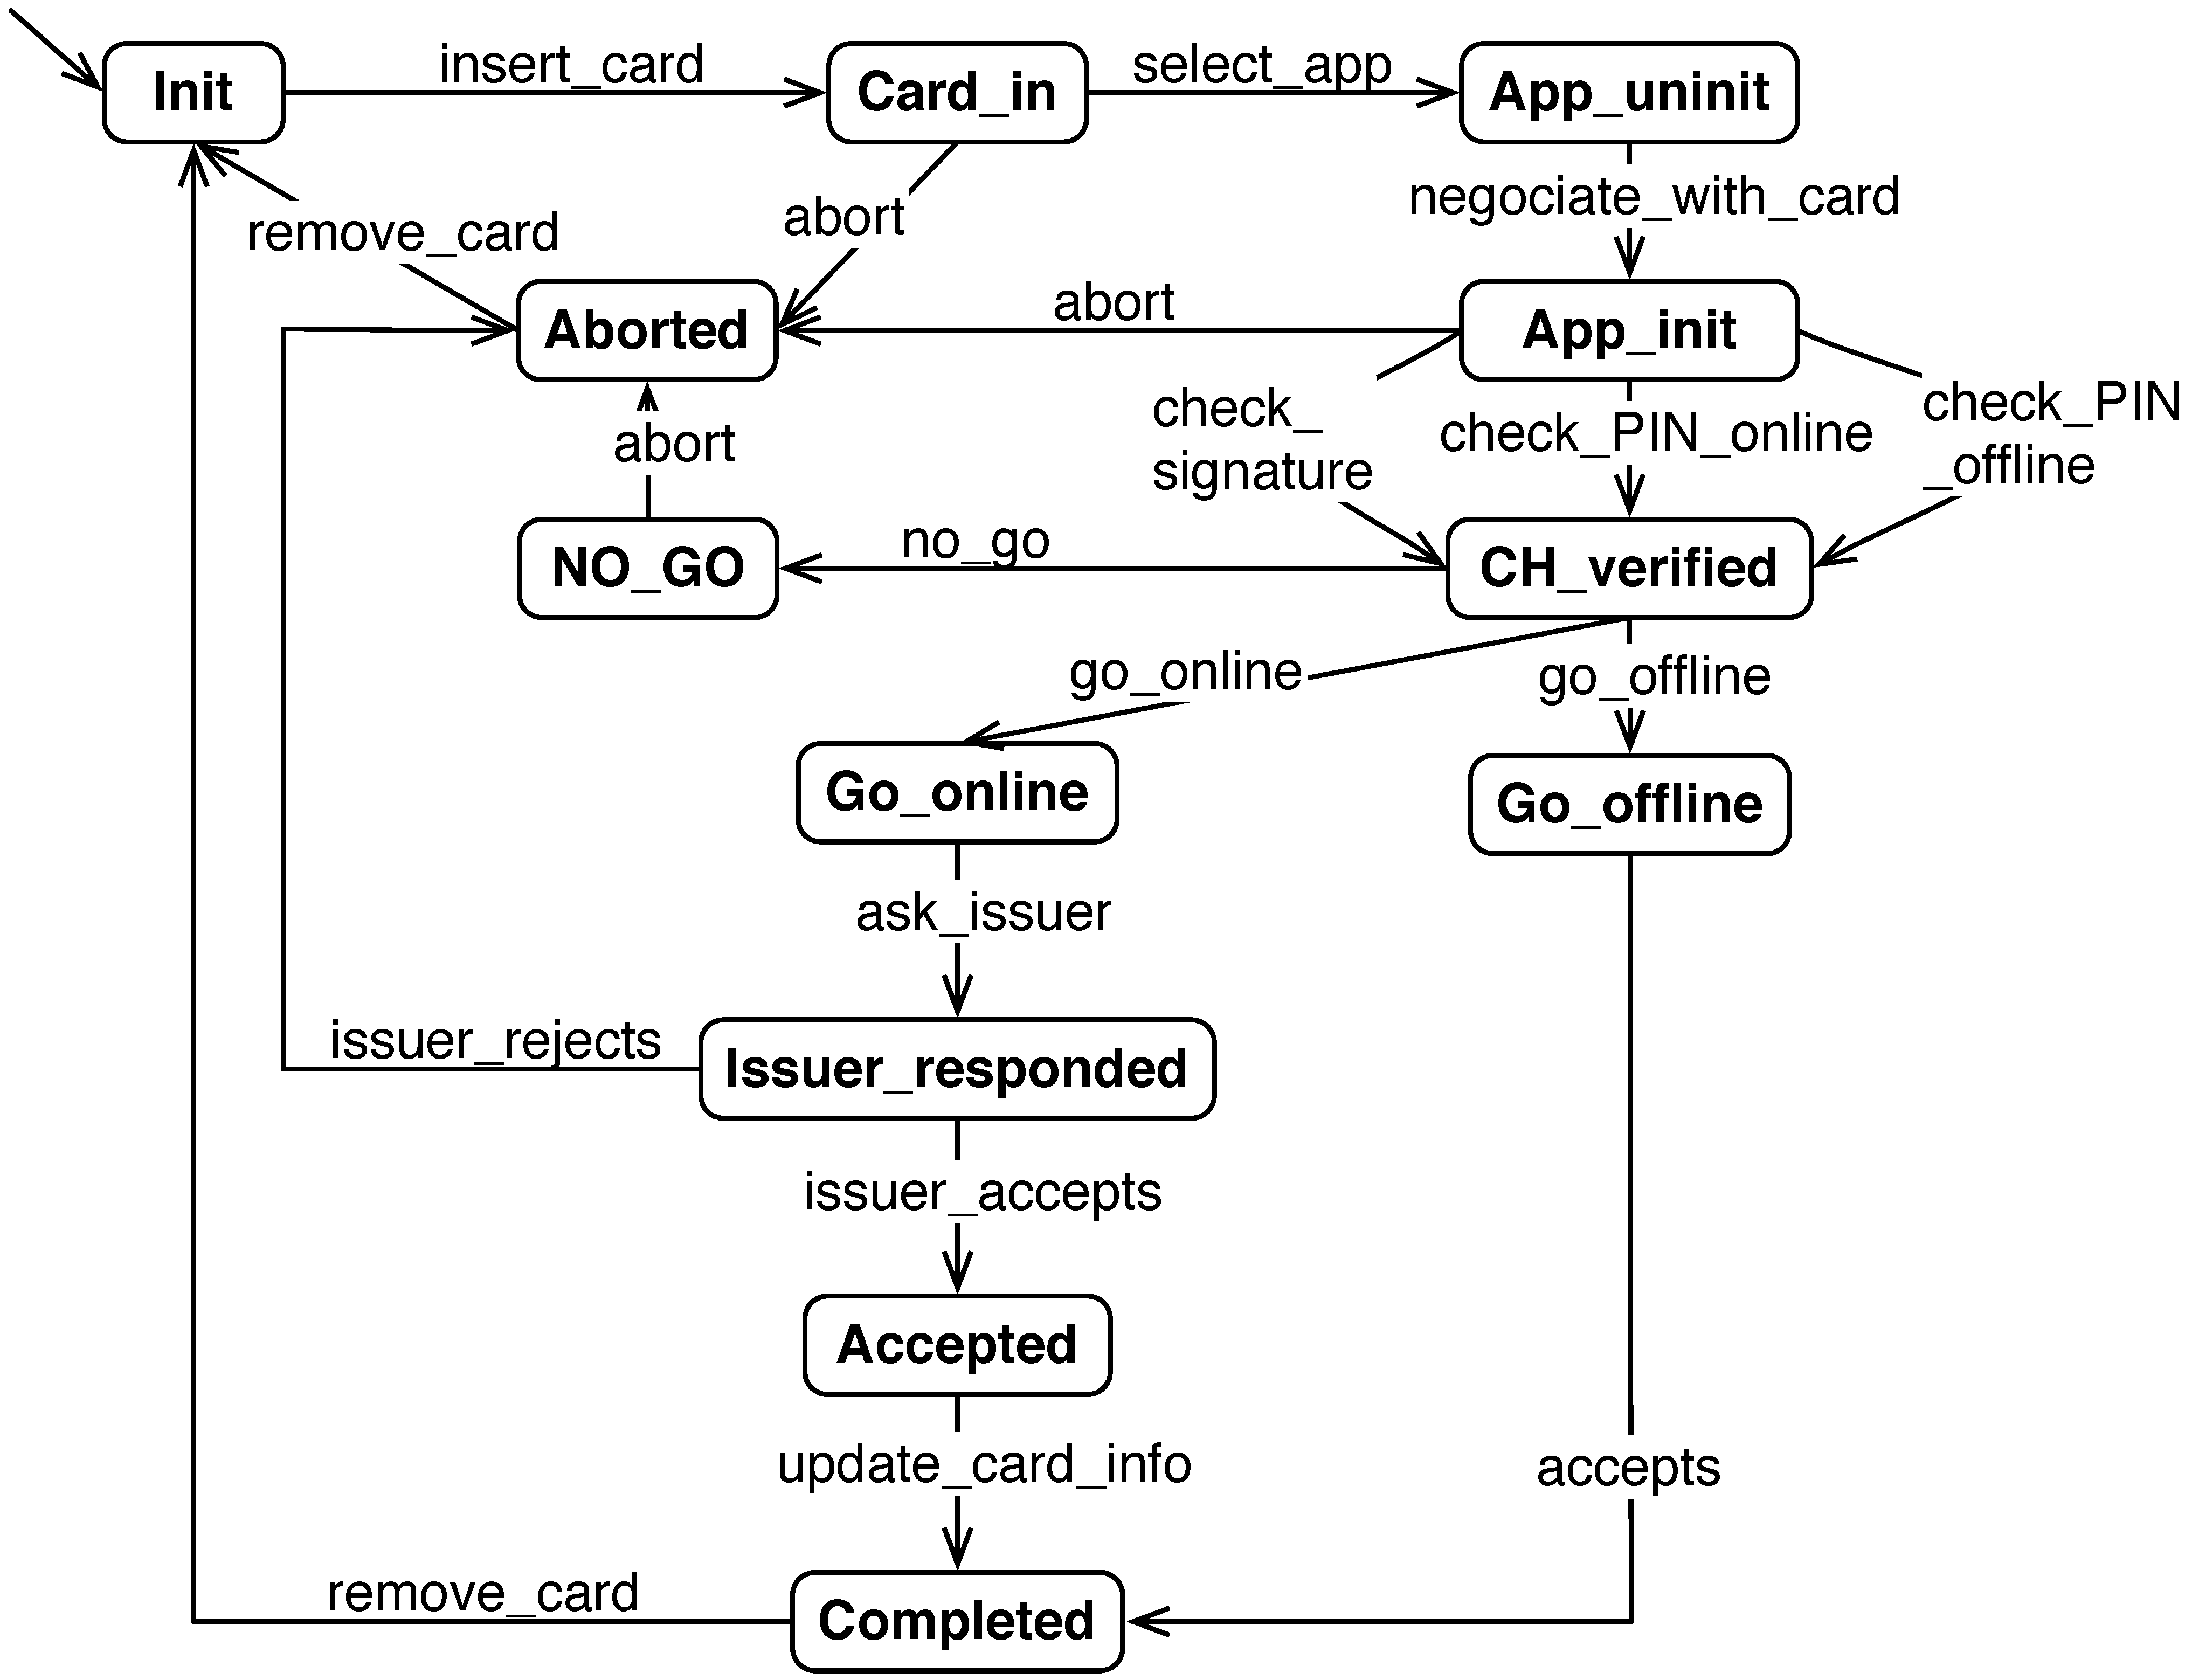
\includegraphics[width=85mm]{card-payment-terminal-product}
	\caption{Card payment terminal product original LTS}
	\label{fig:fmm:cptproduct}
\end{figure}

To address the problems of mutation analysis at the model level, we take our inspiration from our research on software product lines. The idea is to consider mutants as \emph{members} of a \emph{mutants family}\footnote{\textit{Member} is a synonym for \textit{product} or \textit{variant}, and \emph{family} is a synonym for \textit{product line}. For the sake of clarity, we will refer to mutants as \textit{members} of a \textit{mutants family}.}. Considering mutants as part of a family rather than in isolation yields considerable advantages: shared execution at the model level \cite{Classen2013b} and compact representation of a set of mutants. This contrasts with existing product line approaches of mutation analysis \cite{Kim2013a,Nguyen2014,Kim2012a} which require code and hence do not apply to model mutants.

In the following sections, we use as example the specification of one product from the card payment terminal product line described in Section \ref{sec:casestudy:cpterminal}. This product allows both direct debit and credit payments, may perform it online or offline, and allows to identify the card holder using both signature or PIN code. The features from the feature model in Figure \ref{fig:cpterminalfm} selected to form this product are: 
\begin{quote}
$\lbrace$ \textit{CPTerminal, PaymentSchema, DirectDebit, DebitCard, CreditCard, Connectivity, Online, VPN, Offline, CardReader, Chip, MagStrip, Identificator, PIN, Signature} $\rbrace$
\end{quote}
The \gls{LTS} describing the behaviour, obtained using the projection operator on the FTS defined in Figure \ref{fig:cpterminalfts}, is presented in Figure \ref{fig:fmm:cptproduct}.

\begin{figure}[t]
	\centering
	\subbottom[State $\mathit{Go\_offline}$ missing]{
		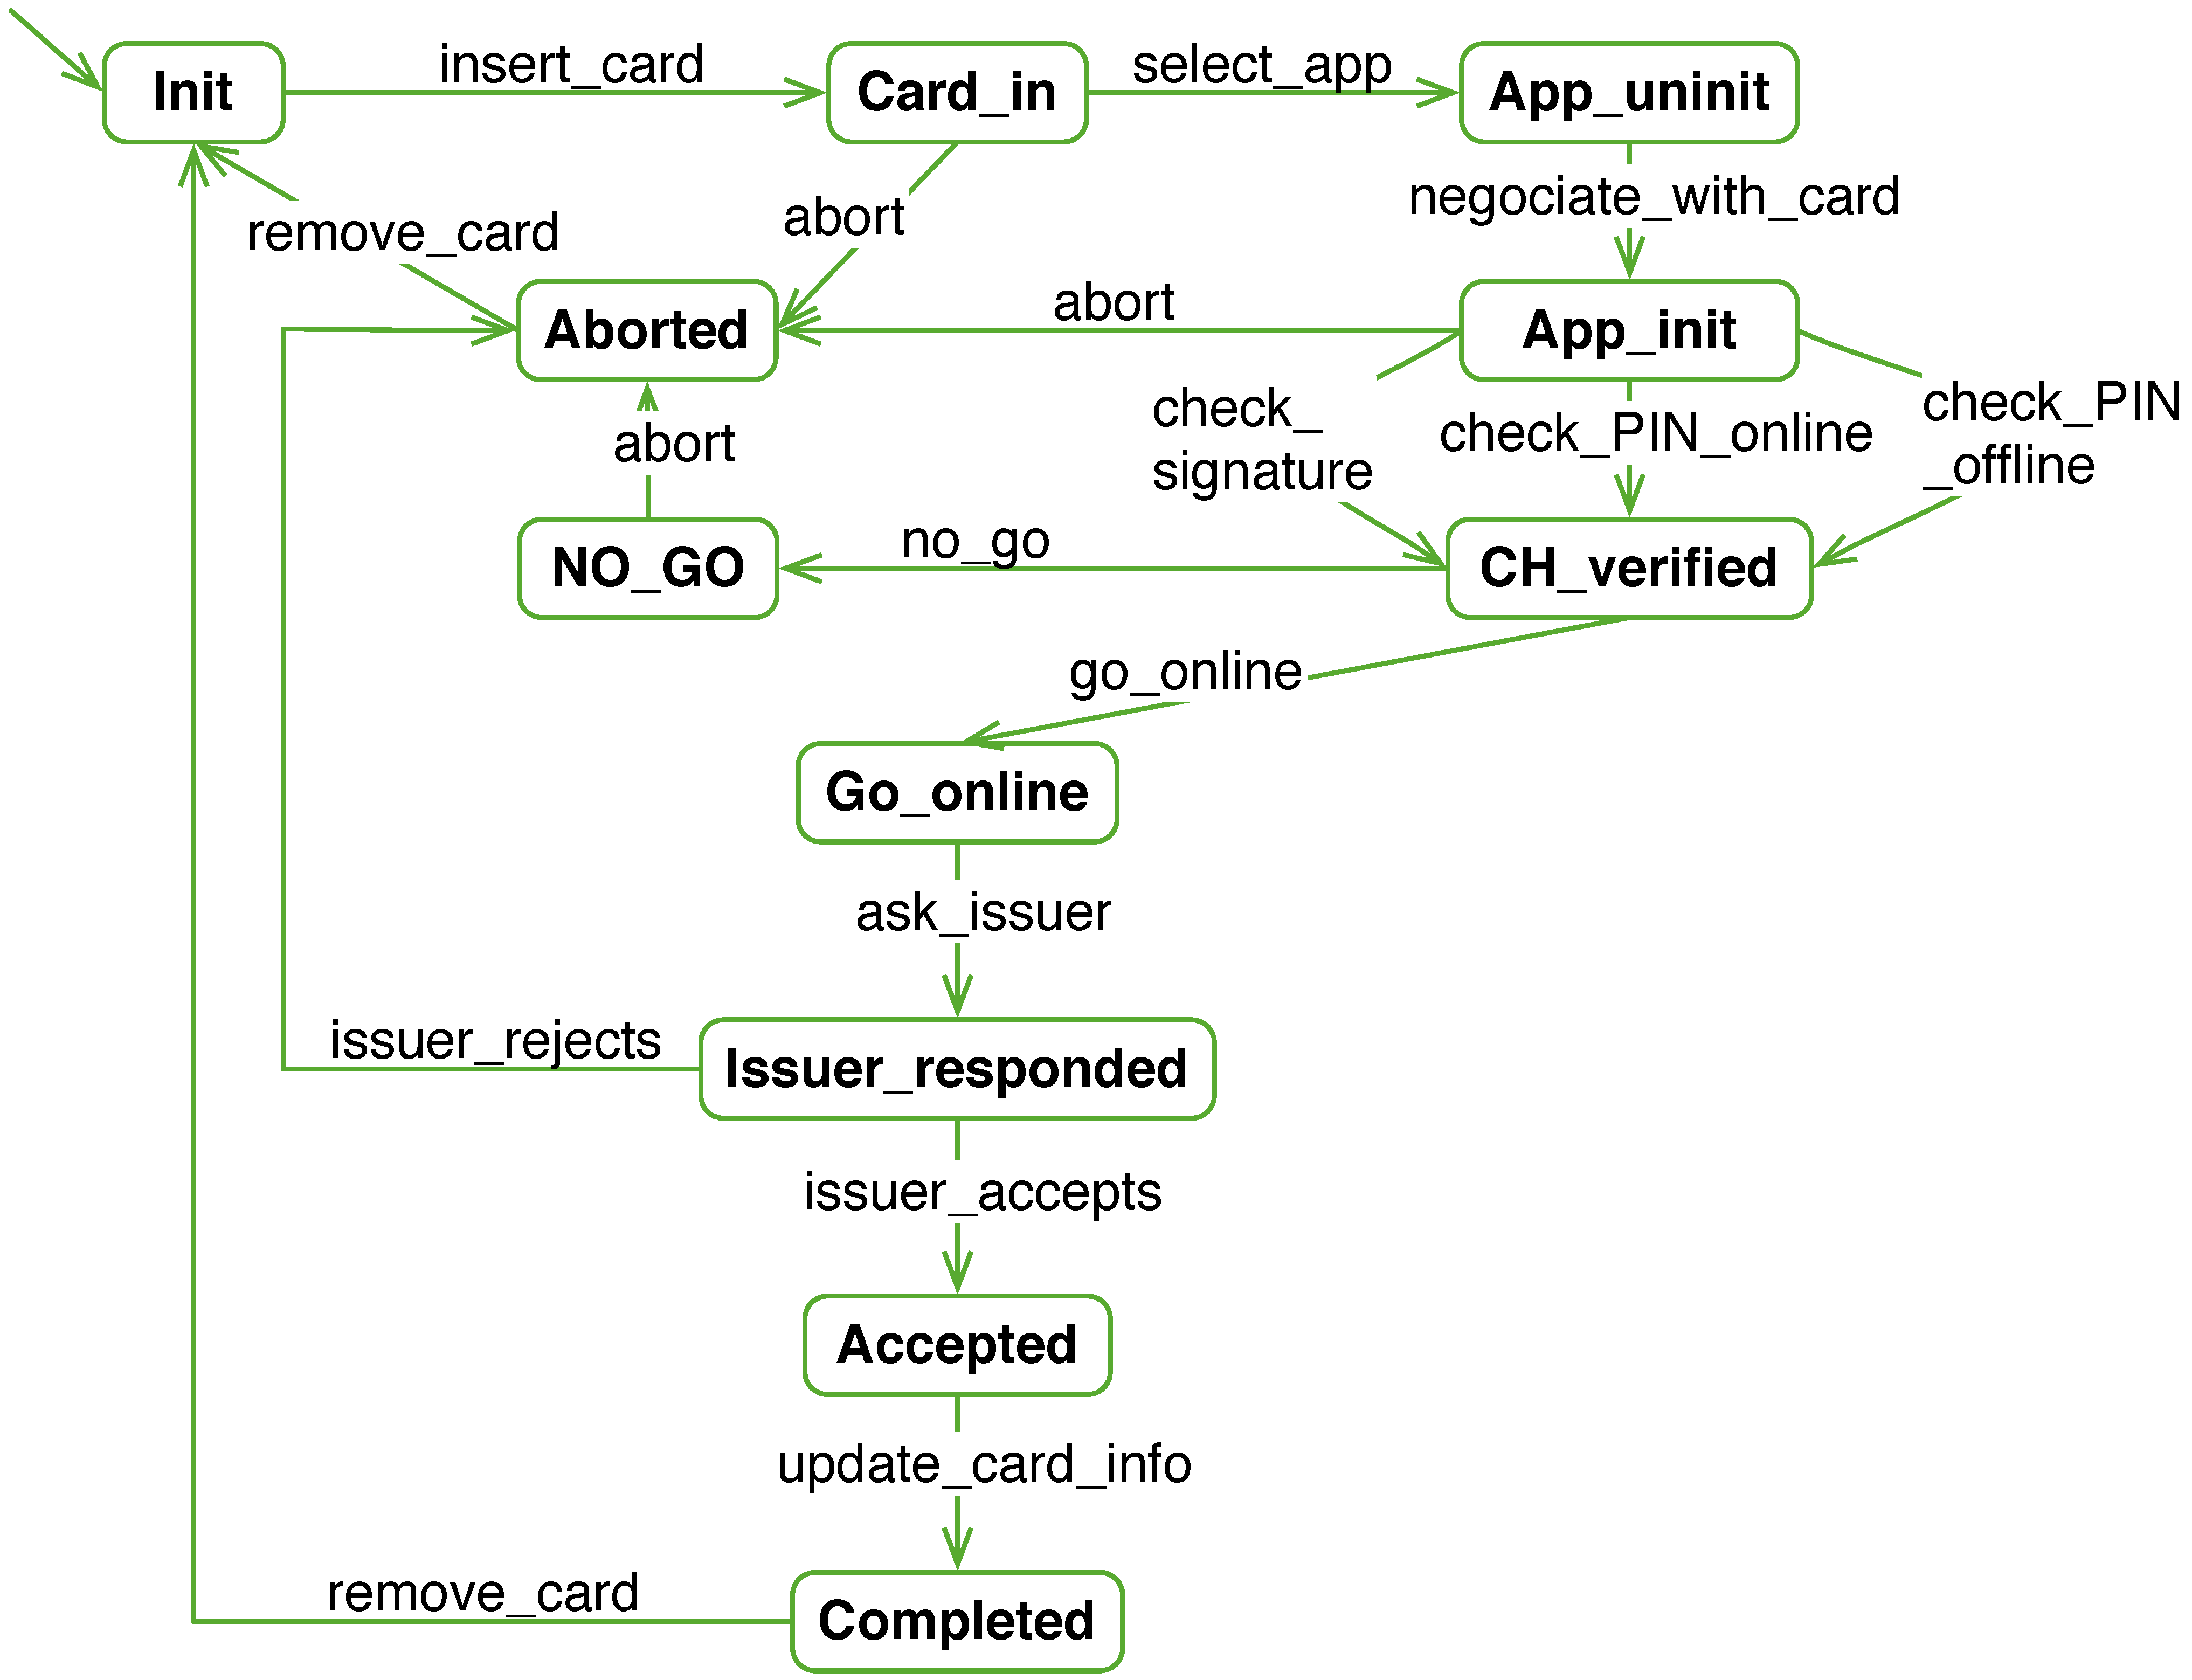
\includegraphics[width=58mm]{cpt-smi_Go_offline}
		\label{fig:fmm:cptsmi}
	}
	\subbottom[State $\mathit{NO\_GO}$ missing]{
		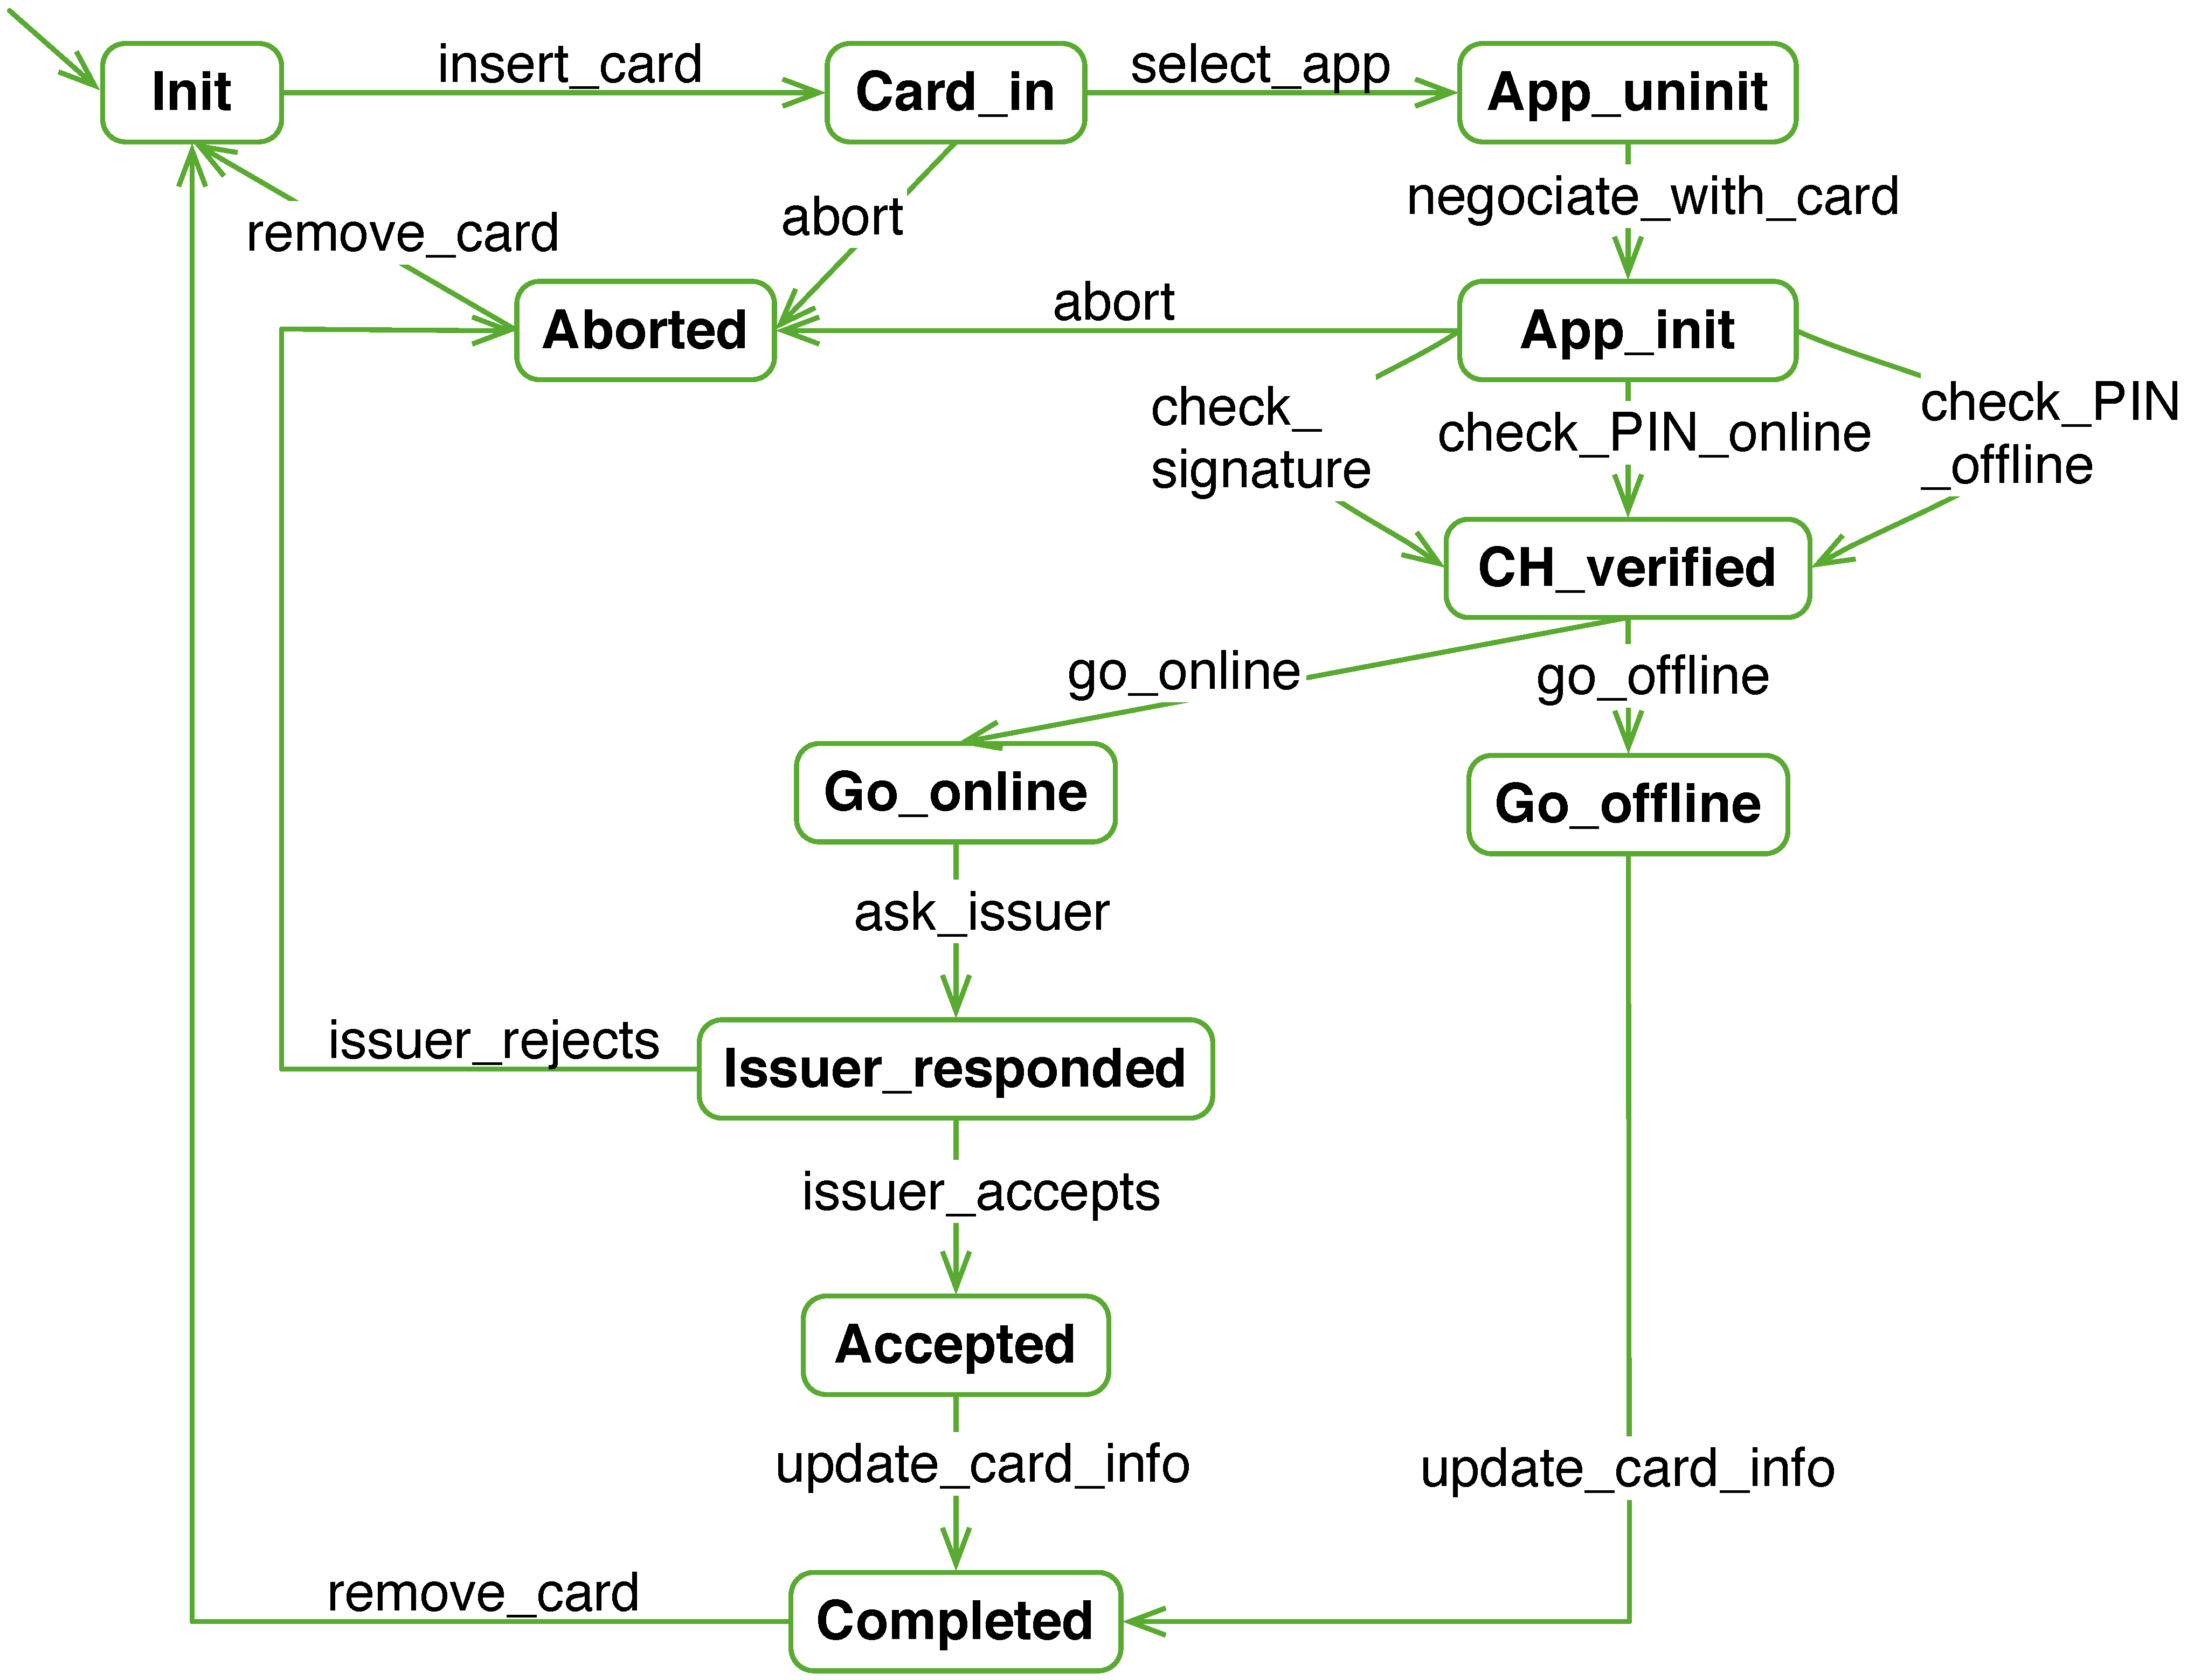
\includegraphics[width=58mm]{cpt-smi_NO_GO}
		\label{fig:fmm:cptsmi2}
	}
	\subbottom[Action $\mathit{issuer\_accepts}$ exchanged]{
		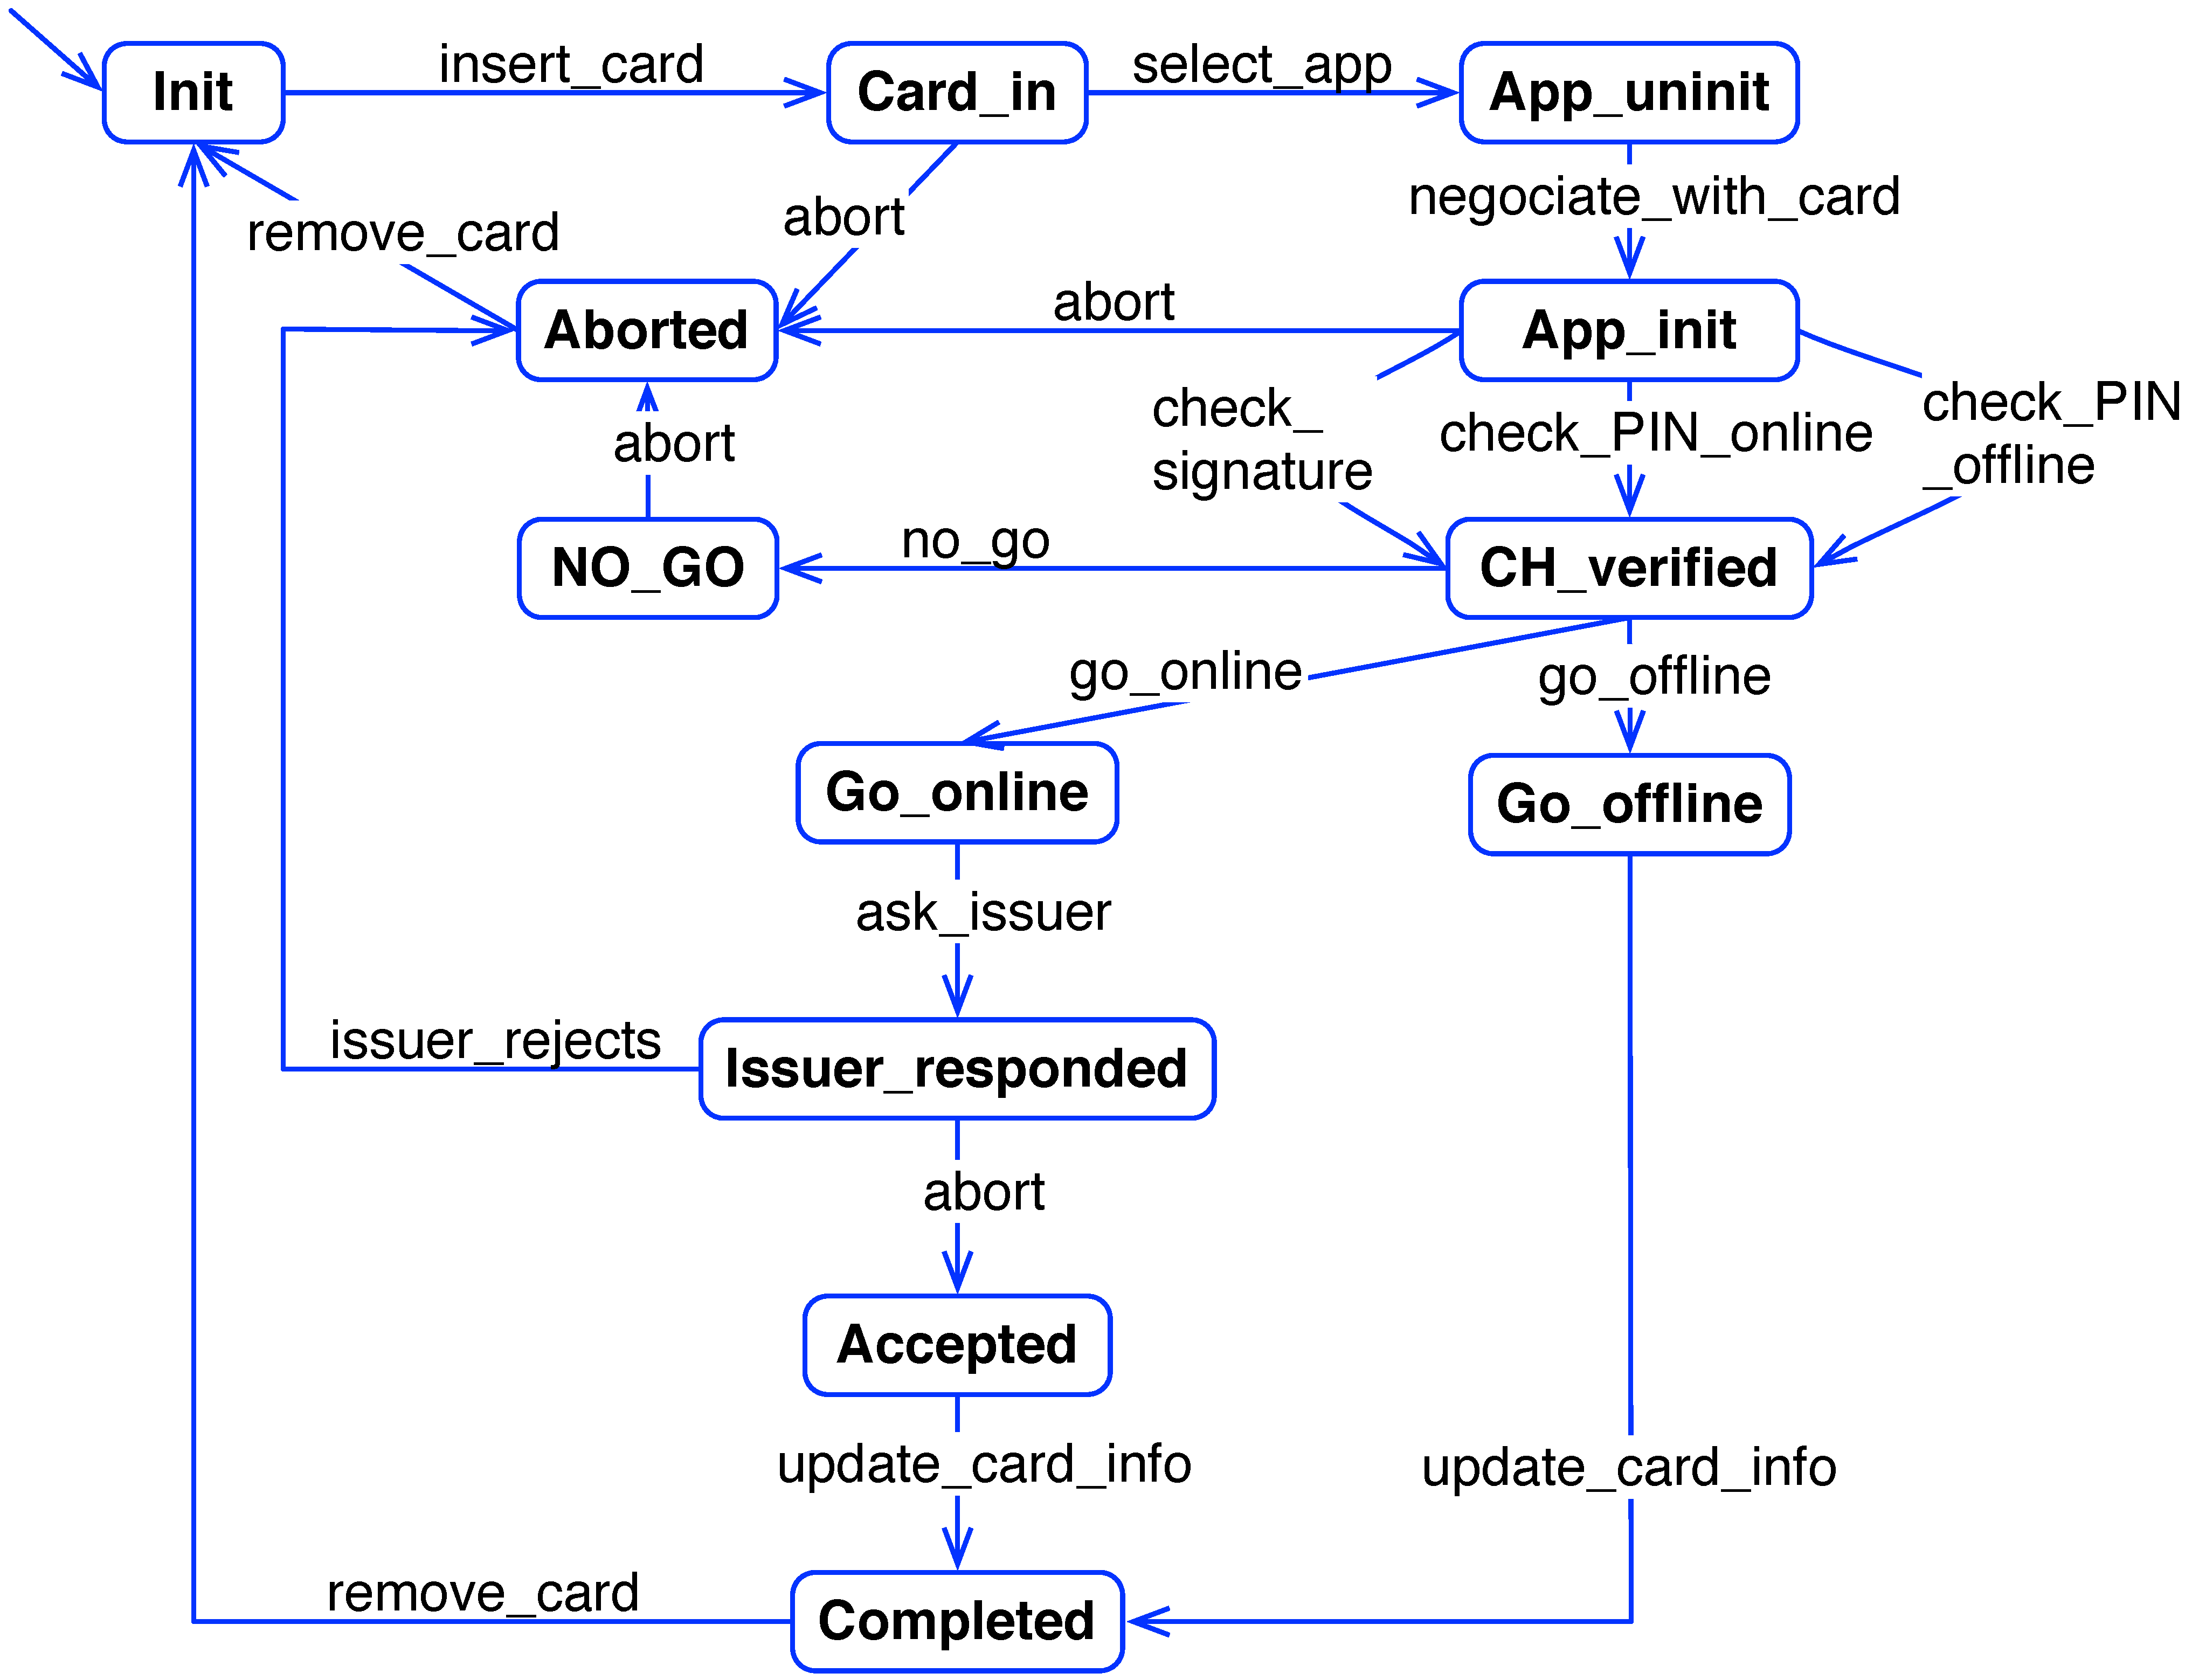
\includegraphics[width=58mm]{cpt-aex_issuer_accepts}
		\label{fig:fmm:cptaex}
	}
	\subbottom[Wrong initial state]{
		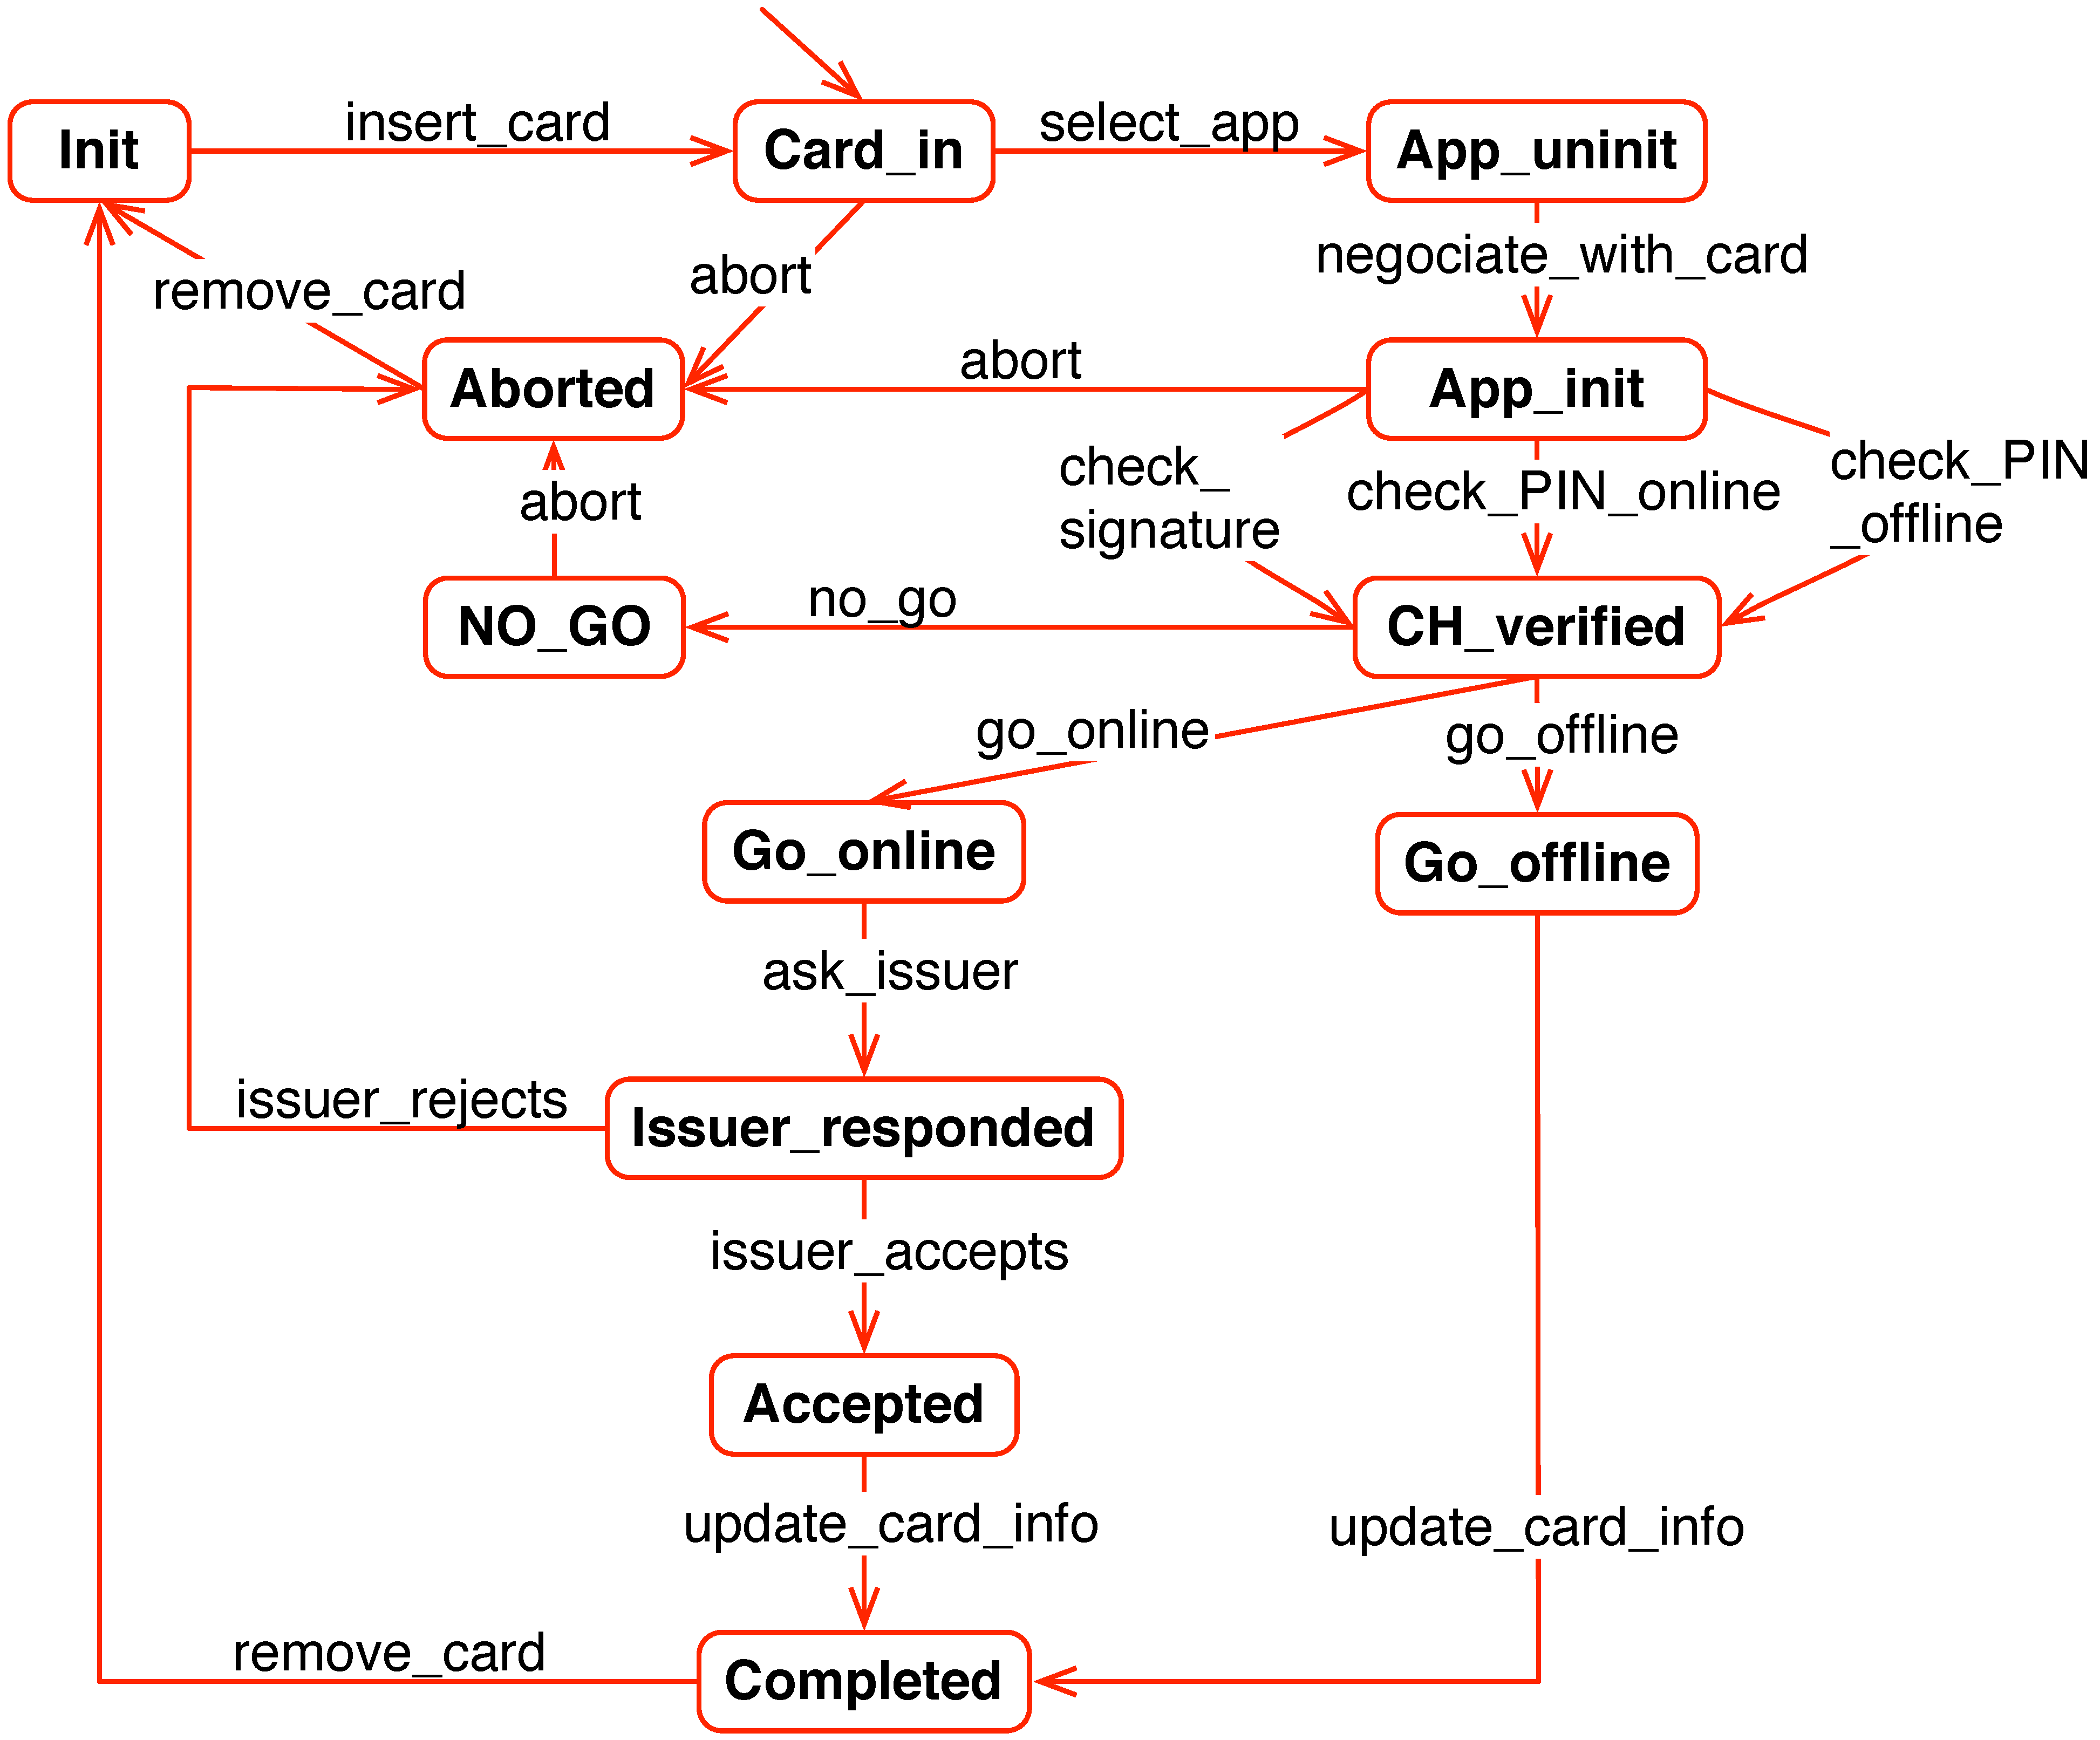
\includegraphics[width=58mm]{cpt-wis_Card_in}
		\label{fig:fmm:cptwis}
	}
	\caption{Card payment terminal product mutants}
	\label{fig:fmm:cptmutants}
\end{figure}

In model-based mutation analysis, mutants are introduced based on model transformation rules, called \emph{mutation operators}, that alter the system specification. Model based mutation is thus a black box testing technique, unlike code-based mutation that requires access to the code and so is white box. An example of mutant obtained from the \textit{state missing operator} applied on the \textit{Go\_offline} state of the card payment terminal system, is presented in Figure \ref{fig:fmm:cptsmi}. There are two kinds of mutants, \textit{first-order} mutants when the original and the mutant models differ by a single model transformation, and \textit{higher order} mutants, derived from the original model after multiple transformations.  

When a mutant is detected by a test case, it is called \emph{killed}. In the opposite situation, it is called \emph{live}. 
In our case, a mutant is killed if a positive abstract test case cannot be executed. For instance, the test case $t_1=( \mathit{insert\_card}$, $\mathit{select\_app},$ $\mathit{negociate\_with\_card},$ $\mathit{check\_PIN\_online},$ $\mathit{go\_offline},$ $\mathit{update}$ $\mathit{\_card\_info},$ \textit{re\-mo\-ve\-\_\-ca\-rd} \textit{)} will kill the mutant of Figure \ref{fig:fmm:cptsmi} since it fails to execute completely. A test case that can be completely executed on a mutant will not detect (kill) it, \eg the test case $t_2=($\textit{insert\_card, select\_app, negociate\_with\_card, check\_PIN\_online, no\_go, abort, remove\_card}$)$ will leave the mutant of Figure \ref{fig:fmm:cptsmi} live because it can be executed completely.

To measure the adequacy of testing, a standard metric called the \emph{mutation score} is used. It is defined as the ratio of mutants killed by the test suite under assessment to the total number of considered mutants. To calculate the mutation score, one has to execute the whole test suite against every selected mutant. In our case, we consider deterministic LTSs and stop the execution of a test case as soon as the LTS is unable to fire the next action. For the test case $t_1$ on the mutant in Figure \ref{fig:fmm:cptsmi}, the execution is stopped when it reaches the $\mathit{CH\_Verified}$ state as it may not execute the next action ($\mathit{go\_offline}$) in $t_1$ and the mutant LTS is considered killed by $t_1$. 
In the following,  we call this approach (\ie executing each test against each mutant model separately), the \emph{enumerative approach}. 


%%%%%%%%%%%%%%%%%%%%%%%%%%%%%%%%%%
\section{Featured mutants model}
%%%%%%%%%%%%%%%%%%%%%%%%%%%%%%%%%%

\label{sec:FMM}

\begin{figure}
	\centering
	\subbottom[Feature model]{
		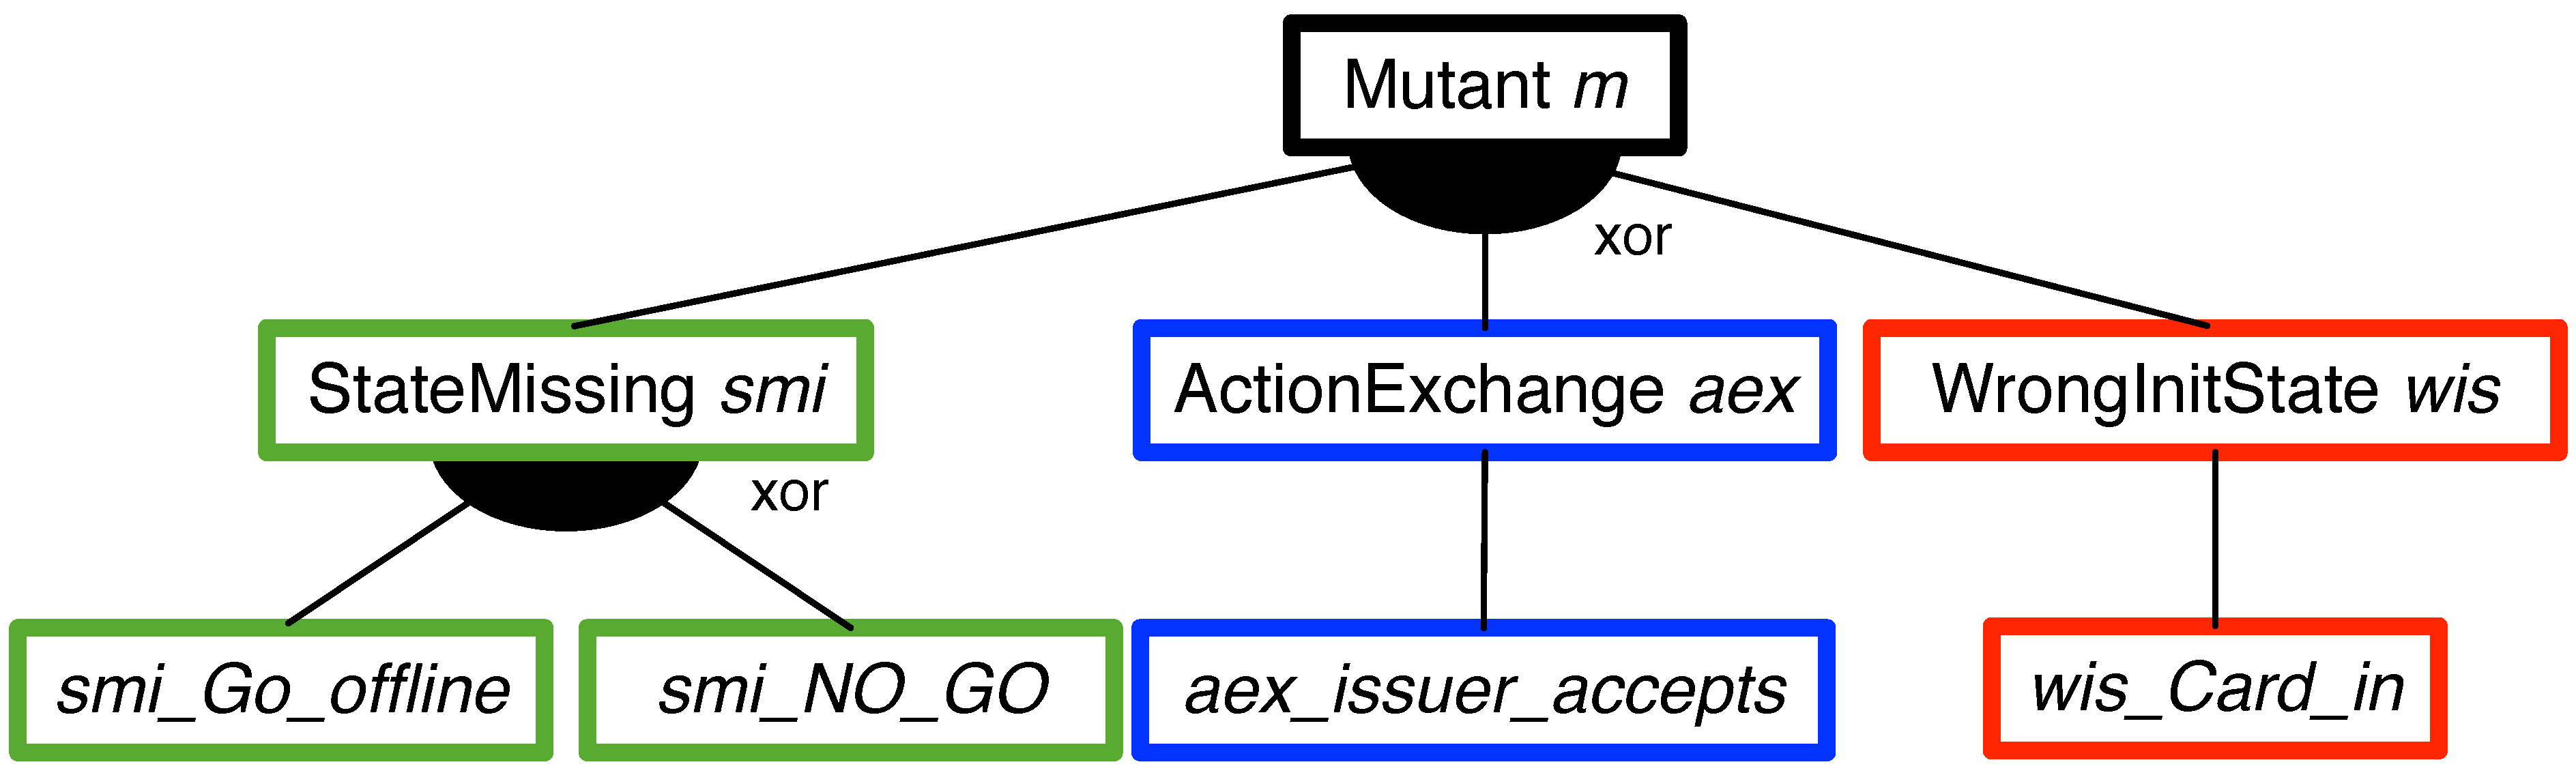
\includegraphics[width=85mm]{cpt-fmm-fm}
		\label{fig:fmm:cptmutantsfm}
	}
	\subbottom[Featured transition system]{
		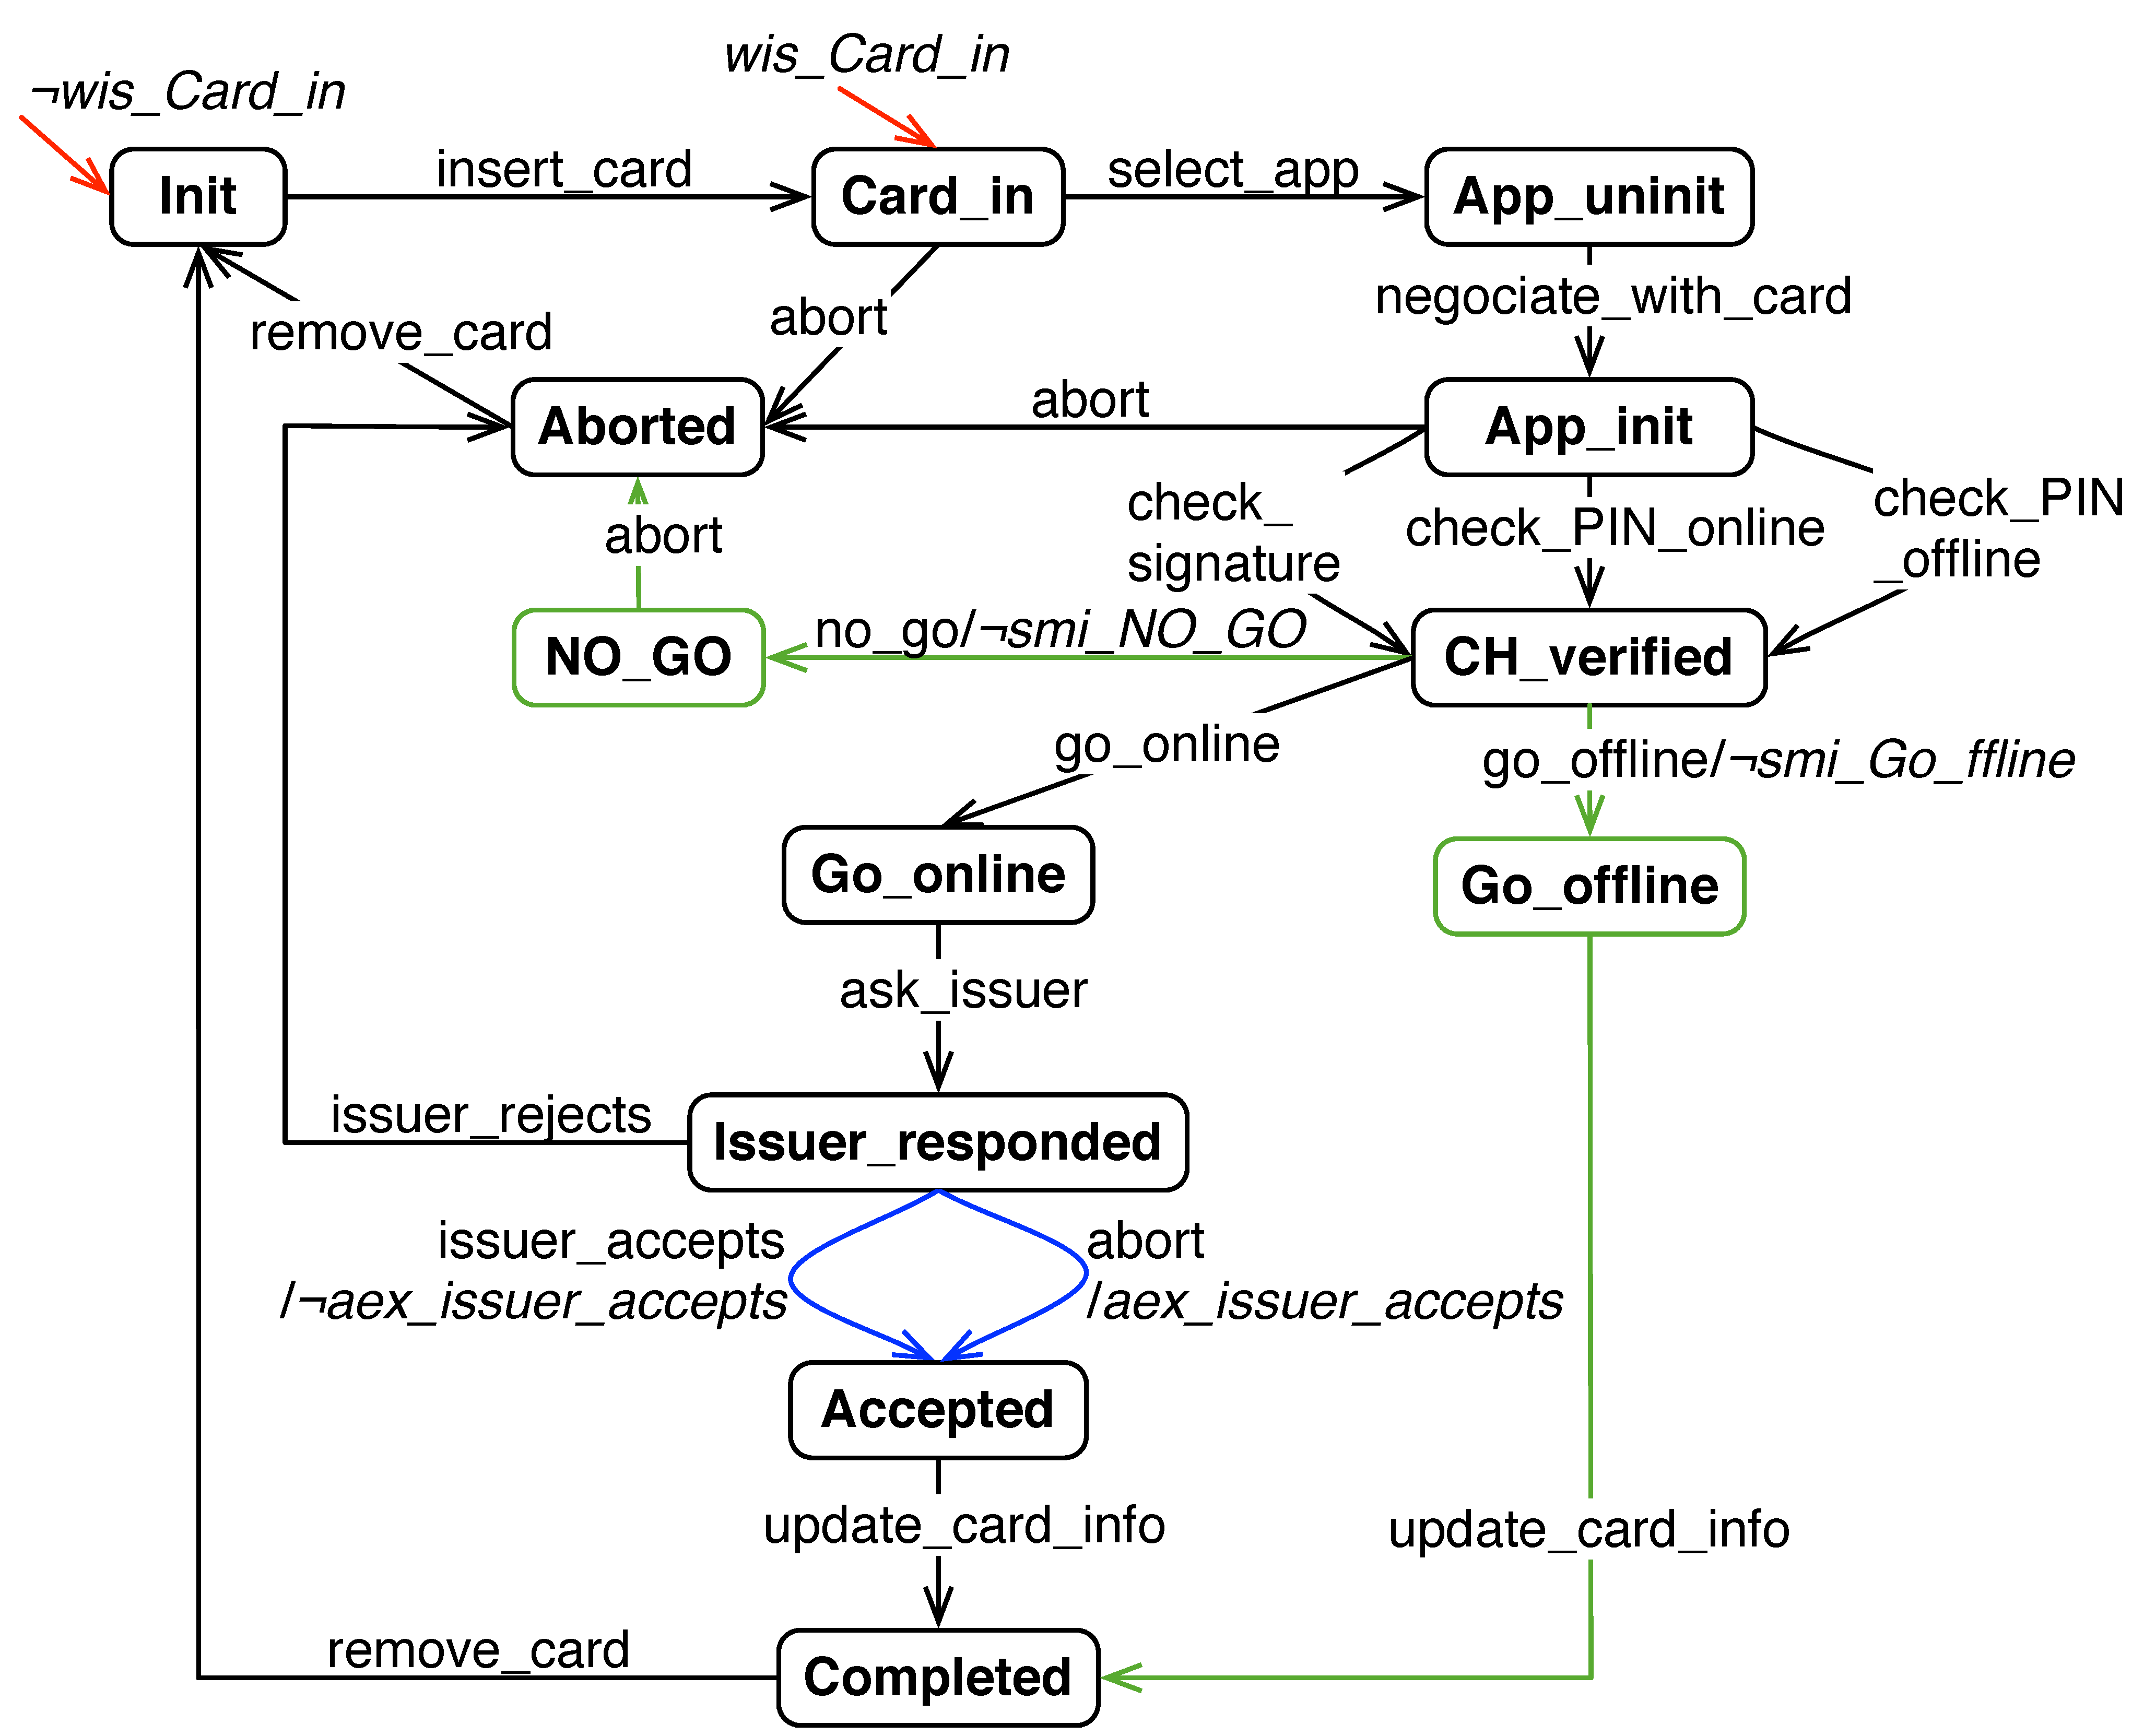
\includegraphics[width=85mm]{cpt-fmm-fts}
		\label{fig:fmm:cptmutantsfts}
	}
	\caption{Card payment terminal product FMM}
	\label{fig:fmm:cptmutantsfmm}
\end{figure}

To represent the variations introduced by the mutation operator (\ie the result of the application of the mutation operator) and the behaviour of the mutants, we use a feature model and an FTS. Each feature in the feature model represents a mutation of the LTS representing the behaviour of the system under test. When a member with one mutation (here represented as a feature) is selected and used with the projection operator on FTS, we obtain the behaviour (represented as a LTS) of the corresponding mutant. This allows us to embed all mutants in a single model, called the \acrfull{FMM}:
%
\begin{definition}[\acrfull{FMM}]
A \gls{FMM} is a couple \textit{(fts,fm)}, where \textit{fts} is an \gls{FTS} representing the behaviour of the original system and all the mutants of the family, and \textit{fm} is its associated \gls{feature model} where each feature represents a mutation of the original system. 
\end{definition}

For example, the FMM of Figure \ref{fig:fmm:cptmutantsfmm} has a feature model in Figure \ref{fig:fmm:cptmutantsfm} with 3 instances of mutation operators: the state missing  (\textit{SMI}) operator, which produces a mutant where one state is missing; the action exchange (\textit{AEX}) operator, which produces a mutant where one transition has its action changed (to another action); and the wrong initial state (\textit{WIS}) operator, which produces a mutant where the initial state has been set to another state. In this instance of the feature model, the SMI operator has been applied twice ($\mathit{smi\_go\_offline}$ mutant presented in Figure \ref{fig:fmm:cptsmi} and $\mathit{smi\_NO\_GO}$ mutant presented in Figure \ref{fig:fmm:cptsmi2}), and the AEX and WIS operators have been applied one time each ($\mathit{aex\_issuer\_accepts}$ mutant presented in Figure \ref{fig:fmm:cptaex} and  $\mathit{wis\_Card\_in}$ mutant presented in Figure \ref{fig:fmm:cptwis}). This feature model represents four first-order mutants, where at most one leaf feature is selected. The FTS in Figure \ref{fig:fmm:cptmutantsfts} represents all the possible variations, corresponding to the four mutation operators, of the original TS.

In order to derive one particular mutant from the FMM, one may use the FTS projection operator. Practically, this operator will first need a valid member of the mutant family, representing the desired mutant, \eg $p = \{m, \mathit{smi}, \mathit{smi\_Go\_offline}\}$; then, each feature expression of the FTS is evaluated with features belonging to the member replaced by true, and other features replaced by false; finally, transitions with a feature expression evaluated to false (\ie where $\gamma p = \mathit{false}$) and states that become unreachable are removed from the FTS. For instance, the projection of the FMM of Figure \ref{fig:fmm:cptmutantsfmm} on $p$ will produce the mutant LTS of Figure \ref{fig:fmm:cptsmi}.

To represent the effect of the WIS operator, we modify the FTS definition (Definition \ref{def:fts}) to replace the initial state $i$ by  a total function $init$ that indicates if a state of the FTS is the initial state of the system: 
%
\begin{definition}[\gls{FTS} for \gls{FMM}]
\label{def:fts4fmm}
A \gls{FTS} is a tuple $(S,$ $\Act,$ $\trans,$ $\mathit{init},$ $d,$ $\gamma)$, where:
\begin{itemize}
\item $S$, $\Act$, $\trans, d, \gamma$ are defined according to definition \ref{def:fts}; 
\item $\mathit{init}:  S \mapsto (\Sem{d} \mapsto \mathbb{B})$ is a total function indicating, for each state, for which product this state is the initial state and defined such that for every product there is exactly one initial state.
\end{itemize}
\end{definition}
%
To be compliant with existing tools, this modification is implemented using an artificial initial state $s_i$, such that for every product, there is an outgoing transition from $s_i$, with no label and a feature expression indicating that this transition may only be fired by this product, and going to the initial state of the product.


%-----------------------------------------------
\subsection{Building the featured mutants model} 
%-----------------------------------------------

\begin{figure}[t]
	\centering
	\subbottom[Enumerative approach]{
		\begin{tabular}{c c}
			\textbf{Input:} $lts$ & \textbf{Output:} $lts_m$ \\
			\begin{tikzpicture}[>=stealth',shorten >=1pt,auto,node distance=2cm]
			  \node[initial,state,initial text=] (s0)				 {$0$};
			  \node[state]         (s1) [right of=s0] {$s_1$};
			
			  \path[->] (s0)  edge node {a} (s1)
			        (s1) edge [bend left] node {a} (s0)
			         	 edge [loop below] node {b} (s1);
			\end{tikzpicture}
			& 
			\begin{tikzpicture}[>=stealth',shorten >=1pt,auto,node distance=2cm]
			  \node[initial,state,initial text=] (s0)				 {$0$};
			  \node[state]         (s1) [right of=s0] {$s_1$};
			
			  \path[->] (s0)  edge node {a} (s1)
			        (s1) edge [bend left] node {\textcolor{blue}{\textbf{b}}} (s0)
			         	 edge [loop below] node {b} (s1);
			\end{tikzpicture}
			\\
		\end{tabular}
		\label{fig:fmm:aexenumapproach}
	}\\
	\subbottom[FMM approach]{
		\begin{tabular}{c c}
			\textbf{Input:} $fts_{fmm}$ & \textbf{Output:} $fts'_{fmm}$ \\
			\begin{tikzpicture}[>=stealth',shorten >=1pt,auto,node distance=2cm]
			  \node[initial,state,initial text=] (s0)				 {$0$};
			  \node[state]         (s1) [right of=s0] {$s_1$};
			
			  \path[->] (s0)  edge node {a/$\gamma_1$} (s1)
			        (s1) edge [bend left] node {a/$\gamma_2$} (s0)
			         	 edge [loop below] node {b/$\gamma_3$} (s1);
			\end{tikzpicture}
			& 
			\begin{tikzpicture}[>=stealth',shorten >=1pt,auto,node distance=2cm]
			  \node[initial,state,initial text=] (s0)				 {$0$};
			  \node[state]         (s1) [right of=s0] {$s_1$};
			
			  \path[->] (s0)  edge node {a/$\gamma_1$} (s1)
			        (s1) edge [bend right=70] node [above] {a/$\neg \mathit{aex} \wedge \gamma_2$} (s0) 
					     edge [bend left] node {\textcolor{blue}{\textbf{b}}/$\mathit{aex}\wedge\gamma_2$} (s0)
			         	 edge [loop below] node {b/$\gamma_3$} (s1);
			\end{tikzpicture}
			\\
		\end{tabular}
		\label{fig:fmm:aexfmmapproach}
	}
	\caption{An example of mutation, the AEX operator}
	\label{fig:fmm:aexexample}
\end{figure}

We rely on the state-of-the-art operators proposed by Fabbri \etal \cite{Fabbri1999} to generate mutants from a LTS:
\begin{itemize}
\item[\emph{SMI}] State Missing operator: removes a state (other than the initial state) and all its incoming/outgoing transitions;
\item[\emph{WIS}] Wrong Initial State operator: changes the initial state;
\item[\emph{AEX}] Action Exchange operator: replaces the action linked to a given transition by another action;
\item[\emph{AMI}] Action Missing operator: removes an action from a transition, leaving an $\epsilon$-transition without action;
\item[\emph{TMI}] Transition Missing operator: removes a transition;
\item[\emph{TAD}] Transition Add operator: adds a transition between two states;
\item[\emph{TDE}] Transition Destination Exchange operator: modifies the destination of a transition.
\end{itemize}
%
Each operator can be used to generate mutants using the enumerative approach, where each mutant is formed as a new variation of the original LTS (possibly introducing non determinism in the case of AEX and TAD operators), or using the FMM approach, where each mutant is an addition to the feature model and the FTS. We detail hereafter the mutant generation procedures (the list of operators and the complete description of their effects is available in Appendix \ref{apdx:fmm:operators}).

\paragraph{Enumerative approach:}
%-------------------------------

\begin{algorithm}
	\KwIn{$\lts$: the original LTS to mutate;\\
		  $\mathit{Ops}$: the set of mutation operators to use;\\
		  $\mathit{times}: \mathit{Op} \rightarrow \mathbb{N}$: a function specifying for each operator the number of applications}
	\KwOut{$\mathit{muts}$, the set of produced mutants}
	\Begin{
		$\mathit{muts} = \emptyset $ \;
		\ForEach{$\mathit{op} \in \mathit{Ops}$}{
			\ForEach{$i \in [1 ; \mathit{times}(\mathit{op})]$}{
				$\mathit{muts} = \mathit{muts} \cup \mathit{op}(\mathit{random}(ts)) $ \; \nllabel{line:fmm:enumgen:mutgen}
			}
		}
  		\Return $\mathit{muts}$\;
	}
	\caption{Mutant generation, enumerative approach}
 \label{algo:fmm:enumgen}
\end{algorithm}

In the enumerative approach, each operator instance (\textit{op}) is defined as a model transformation with input a LTS (\textit{lts}) representing the behaviour of the product. It produces another (mutant) LTS ($\lts_m$) representing the result of this operator instance on $\lts$. For instance, AEX$(s_1, s_0, b)$, shown on Figure \ref{fig:fmm:aexenumapproach}, replaces  the action $a$ on transition $s_1 \overset{a}{\longrightarrow} s_0$ by \textcolor{blue}{$b$}. Algorithm \ref{algo:fmm:enumgen} details the enumerative approach where the set of mutants (\textit{muts}) is produced by applying each operator (in \textit{Ops}) with random parameters a number of times (defined for each operator by the \textit{times} function) on the original LTS (line \ref{line:fmm:enumgen:mutgen}).


\paragraph{FMM approach:}
%------------------------

In the FMM approach, an operator ($\mathit{Op}_{\fmm}$) is defined as a model transformation of a FMM (representing existing mutants), that produces a FMM representing (the previously existing mutants and) the result of the $\mathit{Op_{fmm}}$ mutation \emph{on the original TS} (obtained in the FMM's FTS by replacing the features by false in the feature expressions). 

For instance, in Figure \ref{fig:fmm:aexfmmapproach}, the AEX$_{\fmm}$ operator instance replaces the action $a$ on transition $s_1 \overset{a}{\longrightarrow} s_0$ of the base model by \textcolor{blue}{$b$} as follows: 
\begin{enumerate}
\item adding the feature expression $\neg \mathit{aex}$ on transition $s_1$ $\xrightarrow{a/\gamma_2}$ $s_0$, stating that $s_1$ $\xrightarrow{a/\neg \mathit{aex} \wedge \gamma_2}$ $s_0$ may be fired only if the $\mathit{aex}$ mutation is inactive (and if $\gamma_2$ is true);
\item adding a transition $s_1 \xrightarrow{b/ \mathit{aex} \wedge \gamma_2} s_0$, stating that the transition is fired with a $b$ action only if the $\mathit{aex}$ mutation is active (and if $\gamma_2$ is true);
\item adding an $\mathit{aex}$ feature to $fd_{fmm}$ representing the mutation done by $Op_{fmm}$ (not shown in Figure \ref{fig:fmm:aexfmmapproach}).
\end{enumerate}

\begin{algorithm}
	\KwIn{$\lts$: the original LTS to mutate;\\
		  $\mathit{Ops}$: the set of mutation operators to use;\\
		  $\mathit{times}: \mathit{Op} \rightarrow \mathbb{N}$: a function specifying for each operator the number of applications}
	\KwOut{$\fmm = (\fts_{\fmm}, \fm_{\fmm})$, the FMM}
	\Begin{
		$\gamma = (\lambda t \rightarrow \mathit{true})$ \; \nllabel{line:fmm:fmmmgen:fexprinit}
		$ \fts_{\fmm} = (S, \mathit{Act}, \mathit{trans}, i, \fm_{\fmm},\gamma)$ \; \nllabel{line:fmm:fmmmgen:fmminit}
		$ \fm_{\fmm} = (m) $ \; \nllabel{line:fmm:fmmmgen:fmmfminit}
		\ForEach{$\mathit{op} \in \mathit{Ops}$}{
			\ForEach{$i \in [1 ; \mathit{times}(\mathit{op})]$ \nllabel{line:fmm:fmmmgen:timesop} }{
				$\fmm = \mathit{op}_{\fmm}(\fmm) $ \; \nllabel{line:fmm:fmmmgen:mutgen}
			}
		}
  		\Return $\fmm$\;
	}
	\caption{Mutant generation, FMM approach}
 \label{algo:fmm:fmmgen}
\end{algorithm}

Algorithm \ref{algo:fmm:fmmgen} details the automated FMM building approach. We start with the original LTS and a $\gamma$ function that labels each transition with a true feature expression (line \ref{line:fmm:fmmmgen:fexprinit}). The feature model of the FMM is initialised to a root element $m$ (line \ref{line:fmm:fmmmgen:fmmfminit}). We then apply mutation operators ($\mathit{Ops_{fmm}}$) a specified number of times ($\mathit{times}(\mathit{op})$ line \ref{line:fmm:fmmmgen:timesop}). Contrary to the enumerative approach, the mutation operators are applied on the FMM under construction, which is reused in the next iteration (line \ref{line:fmm:fmmmgen:mutgen}). This is mandatory as the FMM contains all the previous mutations that are taken into account in the model transformations (\eg the $\gamma_{i}$ expressions in Figure \ref{fig:fmm:aexfmmapproach}). 
As we choose to only perform mutations on the original LTS, this forbids operator composition on (previously) mutated elements. Doing so ensures that first-order mutation maps to only one edit of the original LTS and that higher order mutants do not edit the same elements of the original LTS more than once.
Further details about the operators and specificities of the transformations can be found in Appendix \ref{apdx:fmm:operators}.

%-----------------------------------------------
\subsection{Featured mutants model execution}
%-----------------------------------------------

A test case for a product (\ie a LTS) is defined as a sequence of actions in this LTS (\textit{lts}), such that one execution form a path starting from and ending at the initial state (\textit{i}): $t=(\alpha_1, ..., \alpha_n) $ such that $ (i \overset{\alpha_1}{\longrightarrow} s_1, ..., s_{n-1} \overset{\alpha_n}{\longrightarrow} i)$.
Recall that in the enumerative approach, if a test case cannot be executed by the mutant (denoted $m \overset{t}{\nRightarrow}$) or does not end in the initial state of the original LTS (considered as the accepting state), it is considered  killed. Otherwise, the mutant is considered live. The set of live mutants, for $t$ in the set of mutants \textit{muts}, is defined as:
%
$$\mathit{liveEnum}(\mathit{muts}, t) = \{ m \in \mathit{muts} \mid m \overset{t}{\Longrightarrow} i  \} $$
%
In the FMM approach, a test case can be executed on an FMM \textit{fmm} (denoted $\fts_\mathit{{fmm}} \overset{t}{\Longrightarrow}$), if there exists at least one mutant or the product is able to execute it. 
The enumerative approach executes each test case on each mutant separately. In contrast, one execution of a test case on the FMM explores all the reachable mutants (identified by the collected feature expression $\gamma$).
The set of live mutants in the FMM approach is defined as:
%
$$\mathit{liveFMM}(\fmm, t) = \{ p \in [\![\fm_\mathit{{fmm}}]\!] \mid \fts_{\mathit{fmm} \mid p} \overset{t}{\Longrightarrow} i \}$$
%
Concretely, all possible paths in $\fts_\mathit{{fmm}}$ starting from $i$ and ending in $i$ will be considered, which allows to deal with possible non-determinism introduced by a mutation. The live mutants are those able to execute at least one of those paths, \ie those for which the product $p$ satisfies all the feature expressions on the transitions of the considered path.

For instance, the test case:
\begin{align*}
t =  & (\mathit{insert\_card}, \mathit{select\_app}, \mathit{negociate\_with\_card}, \mathit{check\_PIN\_offline},\\
 & \mathit{go\_offline}, \mathit{update\_card\_info}, \mathit{remove\_card})
\end{align*}
Executing the FMM of Figure \ref{fig:fmm:cptmutantsfmm}, it will fire the following transitions:
%
\begin{gather*}
( \xrightarrow{/\neg \mathit{wis\_Card\_in}} \mathit{Init},\\
 \mathit{Init} \xrightarrow{\mathit{insert\_card}} \mathit{Card\_in}, \\
 \mathit{Card\_in}  \xrightarrow{\mathit{select\_app}} \mathit{App\_uninit}, \\
 \mathit{App\_uninit} \xrightarrow{\mathit{negociate\_with\_card}} \mathit{App\_init}, \\
 \mathit{App\_init} \xrightarrow{\mathit{check\_PIN\_offline}} \mathit{CH\_verified}, \\
 \mathit{CH\_verified} \xrightarrow{\mathit{go\_offline}/\neg \mathit{smi\_go\_offline}} \mathit{Go\_offline}, \\
 \mathit{Go\_offline}  \xrightarrow{\mathit{update\_card\_info}} \mathit{Completed}, \\
 \mathit{Completed} \xrightarrow{\mathit{remove\_card}} \mathit{Init}) \\
\end{gather*}
%
These transitions may only be fired by mutants for which all the features expressions are $true$. Here, mutants need to respect the following constraint:
$$\neg \mathit{wis\_Card\_in} \wedge \mathit{\neg smi\_go\_offline}$$
All mutants in the feature model of Figure \ref{fig:fmm:cptmutantsfm} that satisfy this feature expression remain live after the execution of $t$. The set of mutants killed by the test case is computed using the conjunction of $\fm_{\fmm}$ and the negation of this feature expression: $\fm_{\fmm} \wedge (\mathit{wis\_Card\_in} \vee \mathit{smi\_go\_offline})$, which corresponds to the set of mutants: 
$$\left\lbrace(m, \mathit{wis}, \mathit{wis\_Card\_in}), (m, \mathit{smi}, \mathit{smi\_go\_offline}) \right\rbrace$$

In practice, $\mathit{liveFMM}(\fmm, t)$ produces a feature expression representing all the live mutants as detailed in Algorithm \ref{algo:fmm:livefmm}. Initially, the algorithm computes all the paths in $\fts_\mathit{{fmm}}$ corresponding to the sequence of actions in $t$ (line \ref{line:fmm:livefmm:paths}). For one path, the conjunction of the feature expressions gives the mutants able to execute this path (line \ref{line:fmm:livefmm:disjunct}). Effort is saved this way by ignoring unreachable mutants and by sharing the execution of the common transitions. This conjunction disjuncts with the conjunctions of the others paths to get the feature expression representing all the live mutants (line \ref{line:fmm:livefmm:disjunct}). This step results in savings due to merging of the considered executions. For performance reasons, the $\mathit{paths}$ variable uses a tree representation to merge common prefixes of different paths.

\begin{algorithm}
	\KwIn{$\fmm = (\fts_{\fmm}, \fm_{\fmm})$, the FMM;\\
		  $t = (\alpha_1, ..., \alpha_n)$: a test case defined over the original LTS}
	\KwOut{$\mathit{live}$, the feature expression representing the mutants live after executing $t$ on $\fmm$}
	\Begin{
		$\mathit{live} = false$ \;
		$\mathit{paths} = \{ (i \overset{\alpha_1 / \gamma_1}{\longrightarrow}\ldots \overset{\alpha_n / \gamma_n}{\longrightarrow} i) \} $ \; \nllabel{line:fmm:livefmm:paths}
		\ForEach{$p \in \mathit{paths}$}{
			$ \mathit{live} = \mathit{live} \vee (\bigwedge_{\gamma_i \in p} \gamma_i)$ \nllabel{line:fmm:livefmm:disjunct}
		}
  		\Return $\mathit{live}$\;
	}
	\caption{FMM mutant execution}
 \label{algo:fmm:livefmm}
\end{algorithm}

We implemented the different mutant operators described in Appendix \ref{apdx:fmm:operators} in order to perform classical mutation testing (enumerative approach) as well as FMM generation and execution in VIBeS, our Variability Intensive Behavioural teSting Java framework.


%-----------------------------------------------
\subsection{FMMs as higher order mutants model}
%-----------------------------------------------

Higher order mutants can be valuable since some of them tend to be hard to kill \cite{Harman2014}. However, the number of mutants grows exponentially according to the order $n$ and explodes the involved cost. This is obvious in Algorithm \ref{algo:fmm:enumgen}, for the enumerative approach, which generates all the $n-1$ mutants to generate the $n$th-order ones.

Using the FMM approach, modelling higher order mutation comes at (nearly) no cost. In a FMM ($\fts_{\fmm}, \fm_{\fmm}$), the set of allowed mutants (\ie variations in $\fts_{\fmm}$) is represented by the feature model ($\fm_{\fmm}$). For instance, the constraints in the $\fm_{\fmm}$ of Figure \ref{fig:fmm:cptmutantsfm} allows to have exactly one mutant at a time. Meaning that all valid mutants (members) of this FMM will have at most one variation from the original LTS made by a mutation operator, \eg Figure \ref{fig:fmm:cptsmi} has (only) $\mathit{smi\_go\_offline}$ feature active. 

\begin{figure}[h]
	\centering
	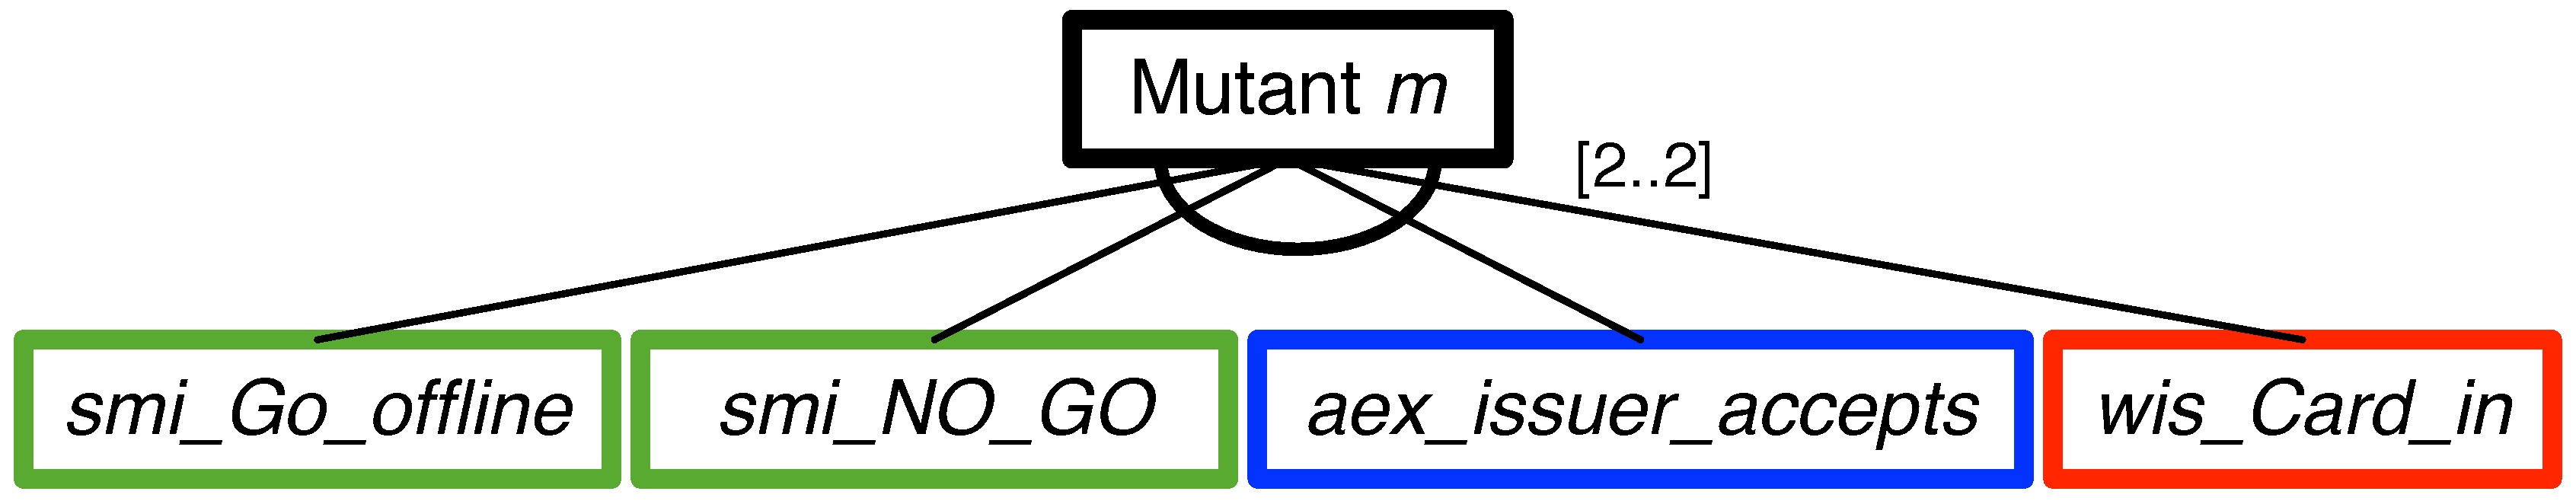
\includegraphics[width=85mm]{cpt-fmm-order2-fm}
	\caption{The order 2 FMM of the card payment terminal example}
	\label{fig:fmm:order2fmm}
\end{figure}

The $n$th order mutants are represented by modifying the constraints on the $\fm_{\fmm}$ so that they have exactly $n$ mutations at a time. It means that generating the FMM using Algorithm \ref{algo:fmm:fmmgen} will also generate the FTS (which will be the same) for order 1 to $n$ FMMs. For instance, the card payment terminal product has the same FTS, for all orders as shown in Figure \ref{fig:fmm:cptmutantsfts}, but differs on the feature model that is described by Figure \ref{fig:fmm:order2fmm} by the group cardinality stating that exactly 2 subfeatures have to be selected. The FMM will compactly represent all the $C^{4}_{2} = 6$ 2nd-order mutants.

\paragraph{All-order mutants:} 
%-----------------------------

Using the same argument, we generalize to mutants of any order by setting the group cardinalities of the feature model in Figure \ref{fig:fmm:order2fmm} to  $[1..4]$. In this case, the FMM represents a single model with all possible orders of mutants (with $n$ between 1 and the number of leaf features in the FMM's feature model). A valid member (mutant) of the feature model will contain at least one application of a mutation operator,\eg a mutant $m = \{m,$ $\mathit{smi\_go\_offline}\}$, but also  $m' = \{m,$ $\mathit{smi\_go\_offline},$ $\mathit{smi\_NO\_GO}\}$, or $m'' = \{m,$ $\mathit{smi\_go\_offline},$ $\mathit{wis\_Card\_in}\}$, \etc In this case, the FMM compactly represent all the $2^{4} - 1 = 15$  $n$-order mutants.

The number of live mutants after the execution of a test case ($t$) on a FMM ($\fmm$) can be obtained by counting the number of SAT solutions (\ie the number of possible assignments for each feature) to $\fm_{\fmm} \wedge \mathit{liveFMM}(\fmm, t)$, where $\fm_{\fmm}$ is the FMM feature model encoded as a boolean formula, \ie the disjunction of the mutations ($\mathit{Ops}$): $\fm_{\fmm} = \bigvee_{o \in \mathit{Ops}} o$. For a test set ($s$), the number of live mutants is computed by counting the number of SAT solutions to
%
$$ \left(\bigvee_{o \in \mathit{Ops}} o \right) \wedge \left(\bigwedge_{t \in s} \mathit{liveFMM}(\fmm, t) \right). $$


%%%%%%%%%%%%%%%%%%%%%%%%%%%%%%%%%%%%
\section{Equivalent mutants problem}
%%%%%%%%%%%%%%%%%%%%%%%%%%%%%%%%%%%%

\label{sec:EMP}

\glsreset{EMP}

Despite its potential, mutation analysis faces a number of challenges that currently prevent wider adoption \cite{Papadakis2015, Jia2011a}. One of them is the \textit{\gls{EMP}}. It concerns the mutants whose behaviour is identical to the original artefact (code or model). Such mutants cannot be distinguished by any test case, a situation that raises two issues: 
\begin{inparaenum}
\item they hamper the use of the criterion as a stopping rule by skewing the mutation score measurement (the number of killed mutants divided by the total number of mutants); and
\item they do not bring any new value to the test selection techniques as they attempt to kill mutants that have no chance to be killed. 
\end{inparaenum}

Mutant equivalence  can take two forms \cite{Papadakis2015}: 
\begin{inparaenum}
\item equivalence between mutants and the original system; \label{item:equivmutants}
\item equivalence between two mutants (not with the original system). \label{item:duplmutants}
\end{inparaenum}
Mutants of case (\ref{item:equivmutants}) are called \emph{equivalent} while mutants of case (\ref{item:duplmutants}) are called \emph{duplicate}. We focus here on mutants that are behaviourally equivalent to the original system, \ie mutants of case (\ref{item:equivmutants}).   

%-----------------------------------------
\subsection{\gls{EMP} and automata theory}
%-----------------------------------------

\glsreset{ALE}

The model-based formulation of the \gls{EMP} can be expressed as a classical problem in automata theory: \emph{\gls{ALE}}. The accepted language of an automaton is formed by all the sequences of actions (words)  that can be accepted \ie starting in the initial state and ending in a final state. Therefore, if a mutant $m$ accepts the same language as the original $o$ (\ie is language-equivalent to the original), then there is no test sequence $s$ that can distinguish the mutant from the original:
$$ \forall s, s \in \mathcal{L}(o) \Leftrightarrow s \in \mathcal{L}(m)$$

There are various relations defined between two automata that we can compute to determine whether they are language-equivalent. Among them, we can cite bisimulations or trace equivalence \cite{Baier2008}. In the last years, the verification community came up  with dedicated relations concepts such as bisimulations up to congruence \cite{Bonchi2013} or antichains \cite{Doyen2010} to address language equivalence.  In model-based mutation testing, Aichernig \etal investigated  language inclusion (but not equivalence) using refinement checking \cite{Aichernig2015} in order to select mutant-killing test cases.  

Although tackling the language equivalence and inclusion problems from different angles and heuristics, all these techniques may face exponential blow-up since both language inclusion and equivalence were demonstrated to be PSPACE complete \cite{Kupferman1996}. While worst-case complexity can seem discouraging, various heuristics have been proposed to limit the effects of this complexity in practice.  One of our goals is to determine the applicability of an exact language equivalence algorithm to address the EMP \cite{Bonchi2013}. The algorithm selected due to its availability, reported performance over the state of the art and ability to handle non-determinism that mutations may incur. In the next section, we also present two baseline algorithms that run generated traces to distinguish original and mutants' behaviours.

%-----------------------------------------
\subsection{Strong and weak mutation}
%-----------------------------------------

J{\"o}bstl \cite{Jobstl2014} discussed the conditions, identified by DeMillo and Offutt \cite{DeMillo1993}, that must be fulfilled to kill a mutant:
\begin{enumerate}
\item ``the \emph{necessity condition} says that the state of the mutated program after some execution of the mutated statement must be incorrect with respect to the original program. This implies that the mutated statement must be reached. This is necessary, but not sufficient'';
\item ``the \emph{sufficiency condition} says that the final state of the mutant must differ from the final state of the original program, \ie the necessary incorrect intermediate state must propagate to an incorrect final state.''
\end{enumerate}
Satisfying the necessity condition  alone is referred to as \emph{weak mutation}, while satisfying both is \emph{strong mutation} \cite{Howden1982,Mathur2008}. 

\glsreset{WM} \glsreset{SM}

At the model level, our simulations detect an incorrect state if an abstract test case that is valid with respect to the original LTS, is invalid on the mutant LTS, or vice-versa. Indeed, when executed, an abstract test case induces one or more \textit{runs} (alternating sequences of states and actions), depending on the presence of non-determinism. If one run does not contain all the actions of the abstract test case (\ie the run is \emph{incomplete}), it is because of the presence of an incorrect state preventing the subsequent actions to be fired. If all runs are complete, the original and the mutant are assumed equivalent for this test case. 
Necessity and sufficiency conditions affect the final states of these runs. For \gls{WM}, these states can map to any state of the LTS (like for abstract test cases). For \gls{SM}, we need to account for the fact that LTSs have no final states: in this case, we assimilate the initial state to a final state and consider only positive (or negative) abstract test cases for strong mutation.

The \gls{ALE} approach uses automata that have explicit initial and final states. For weak mutation, we generate automata in which all states are final, and for strong mutation the initial state is the only final state.

%-----------------------------------------
\subsection{Mutant equivalence analysis}
%-----------------------------------------

\glsreset{RS} \glsreset{BS}

As explained in the previous sections, equivalent mutant detection may be done using automata language equivalence. Since this is a PSPACE complete problem, we also propose two randomized approaches: \emph{\gls{RS}} and \emph{\gls{BS}}. Those approaches are straightforward:  we generate random (either fully random or biased random) traces from the original (resp. mutant) model and run them on the mutant (resp. original) model. If a trace fails to execute on one of the models, it serves as a counterexample and disproves equivalence.  Otherwise, the mutant is considered \emph{probably equivalent} and testers have to decide whether they want to perform more simulations or switch to an exact method. 

\paragraph{Automata language equivalence:}
%-----------------------------------------

The \gls{ALE} approach we selected for comparison is developed by Bonchi and Pous \cite{Bonchi2013}. It can be thought of as an extension to non-deterministic LTSs of the Hopcroft-Karp algorithm. In particular, they introduce a bisimulation relation called \emph{up to congruence} that requires to explore less states than the original algorithm. This approach also avoids to build the complete deterministic finite TS and performs determinisation on-the-fly. This makes such an approach particularly relevant: non-determinism may be introduced locally by mutations (our original models are deterministic), thereby limiting determinisation scope\footnote{This is indeed the case in our evaluation: between 0\% and 15.5\% of the mutants are non-deterministic (see Section \ref{sec:experiment:mutequiv}).}.

\paragraph{Randomized simulations:}
%-----------------------------------------

\newcommand{\wValid}{\mathit{valid}}
\newcommand{\wInvalid}{\mathit{invalid}}
\newcommand{\wTraceset}{\mathit{traceset}}
\newcommand{\wSelect}{\mathit{select}}
\newcommand{\wNone}{\mathit{none}}

\begin{algorithm}
	\KwIn{$o$, the original LTS;\\
		  $m$, the mutant to compare to $o$; \\
		  $N$, the total number of traces to generate;\\
		  $k$, the length of the abstract test cases;
		 }
	\KwOut{$t$, an abstract test case differentiating $m$ from $o$ or $\wNone$ if $m$ is potentially equivalent to $o$.}
	\Begin{
		$\wTraceset = \wSelect(o, \dfrac{N}{2}, k)$ \; \nllabel{line:fmm:randomequiv:posrandomselect}
		\ForEach{$t \in \wTraceset$}{
			\If{$\neg (m \overset{t}{\Longrightarrow})$ \nllabel{line:fmm:randomequiv:posexec}}{
				\tcp{mutant fails to execute $t$, returns $t$}  
				\Return $\wValid(t)$ \; \nllabel{line:fmm:randomequiv:returnpos}
			}
		}
		$\wTraceset = \wSelect(m, \dfrac{N}{2}, k)$ \; \nllabel{line:fmm:randomequiv:negrandomselect}
		\ForEach{$t \in \wTraceset$}{
			\If{$\neg (o \overset{t}{\Longrightarrow})$ \nllabel{line:fmm:randomequiv:negexec}}{
				\tcp{original LTS fails to execute $t$, returns $t$} 
				\Return $\wInvalid(t)$ \; \nllabel{line:fmm:randomequiv:returnneg}
			}
		}
  		\Return $\wNone$\; \nllabel{line:fmm:randomequiv:return}
	}
	\caption{Mutant equivalence analysis: generic randomized simulation}
 \label{algo:fmm:randomequiv}
\end{algorithm}

Algorithm \ref{algo:fmm:randomequiv} presents our generic randomized simulation approach: $N$ abstract test cases are selected (respectively) from the original model (line \ref{line:fmm:randomequiv:posrandomselect}) and the mutant model (line \ref{line:fmm:randomequiv:negrandomselect}), and executed (respectively) on the mutant model (line \ref{line:fmm:randomequiv:posexec}) and the original model (line \ref{line:fmm:randomequiv:negexec}).  In case of non deterministic behaviour, all the possible paths are considered for the execution of the abstract test case. If one equivalence test fails, the algorithm stops and returns an abstract test case, either valid for the original LTS (line \ref{line:fmm:randomequiv:returnpos}), such as 
$$(o \overset{t}{\Longrightarrow}i) \wedge \neg (m \overset{t}{\Longrightarrow}i)$$ 
or an abstract test case, invalid for the original LTS (line \ref{line:fmm:randomequiv:returnneg}), such as 
$$\neg (o \overset{t}{\Longrightarrow}i) \wedge (m \overset{t}{\Longrightarrow}i)$$

This generic simulation algorithm is instantiated through two strategies for trace generation (lines \ref{line:fmm:randomequiv:posrandomselect} and \ref{line:fmm:randomequiv:negrandomselect}): \acrfull{RS} and \acrfull{BS}. The parameter $N$ is computed using the Chernoff-Hoeffding bound.

\paragraph{Random simulation:}
%-----------------------------

Random simulation assumes a uniform distribution of on the transitions enabled in each state, that is, such abstract test cases are selected randomly ($\wSelect$ call on lines \ref{line:fmm:randomequiv:posrandomselect} and \ref{line:fmm:randomequiv:negrandomselect} in Algorithm \ref{algo:fmm:randomequiv}) by accumulating the actions $\alpha_i$ triggered by a random walk of a given length $k$ in the LTS. For weak mutation (\gls{WM} \gls{RS}), the only constraint is to start the random walk from the initial state $i$. Strong mutation (\gls{SM} \gls{RS}) requires a random walk starting from and ending in $i$\footnote{After few tries, this method (\ie using a random walk until the initial state $i$ is reached) showed very poor results on our largest models (we set a timeout of one hour for one equivalence detection) and is therefore not further discussed. See Section \ref{sec:experiment:mutequiv} for more details.}.


\paragraph{Biased simulation:} 
%----------------------------

The \acrfull{BS} approach exploits the basic characteristics of mutation testing: mutations are localised and they create (most of the time) behavioural differences. It assumes that those differences are detected by an abstract test case $t$ which, when executed on the original LTS $o$ or on its mutant $m$, goes through one of the states affected by the mutation. For instance, the \textit{transition missing operator} produces a mutant by removing a transition $a\overset{\alpha_i}{\longrightarrow}b$ from the original LTS. The \gls{BS} approach (that does not know which mutation has been performed) selects abstract test cases in $o$ and $m$, such that their executions $m \overset{t}{\Longrightarrow}$ or $o \overset{t}{\Longrightarrow}$ reach $a$ or $b$ (where a syntactic difference between the models is detected).  Such states, called \emph{infected states}, have been shown to help identifying equivalent mutants at the code level \cite{Offutt1997,Bardin2015} and to speed up mutation analysis at the model level \cite{Krenn2016}. This motivates us to adopt this strategy in our biased simulation.  

In practice, the set of infected states $S_{\mathit{infect}}$ is computed by checking syntactic differences between the original and mutant LTSs. It will include: 
\begin{enumerate}
\item connected states (\ie states accessible from the initial state) from one model which are not present in the other, 
and
\item states with differences in their input/output transitions: in number of transitions or in action names, considering any pair of states $<s_o,s_m>$ where $s_o$ is a state in the original TS, $s_m$ a state in the mutant TS, such that their names are identical. 
\end{enumerate}
An alternative is to instrument the mutant generator to keep track of the list of infected states while generating the mutants. Our goal is to be able to apply this strategy without any information on how the mutants are generated (\eg generated by other frameworks than ours) and to fairly compare  with an exact approach  that makes no assumption on the locality of differences. Once the set of infected states  $S_{\mathit{infect}}$ is obtained (by any means), the second step is to generate traces that cover such infected states.

For weak mutation (\gls{WM} \gls{BS}), an abstract test case $t$ is selected ($\wSelect$ call on lines \ref{line:fmm:randomequiv:posrandomselect} and \ref{line:fmm:randomequiv:negrandomselect} in algorithm \ref{algo:fmm:randomequiv}) by concatenating the actions of the shortest walk from the initial state $i$ to a randomly chosen state $a \in S_{\mathit{infect}}$ and a random walk starting from $a$. To proceed, the first step during abstract test case selection is to compute the shortest distance (\ie the number of transitions) between each state of the original LTS $o$ (or its mutant $m$ respectively) and the initial state $i$ of $o$ (or $m$ respectively) using a standard breadth-first search \cite{Cormen2001}. 

For strong mutation (\gls{SM} \gls{BS}), instead of a random walk starting from $a$, the algorithm will consider the actions of a path starting from $a$ and returning to $i$ using the computed shortest distance: the distance from $a$ to $i$ will (not strictly) decrease each time a transition is taken in the path.

\paragraph{Estimating the number of required runs:}
%-------------------------------------------------

An important parameter for simulation is the number of abstract test cases selected from the original (resp. mutant) model and run on the mutant (resp. original) model: $N/2$. Under the hypothesis that abstract test cases are uniformly distributed we can bound the equivalence probability and estimating the number of runs needed achieve these bounds. Herault \etal \cite{Herault2004} suggested to use the Chernoff-Hoeffding bound to estimate the number $N/2$ of required runs to limit the equivalence probability depending on the approximation parameter $\epsilon > 0$ and a confidence parameter $\delta < 1$. If $N/2 \geq \frac{4\log(2/\delta)}{\epsilon^2} $ then we have: 
$$Pr \left[ equiv(m,o) \right] = Pr\left[ \left| \frac{A}{N/2}-p \right| \leq \epsilon \right] \geq 1-\delta$$
Where $A$ is the number of successful runs that is either $m \overset{t}{\Longrightarrow}$ or $o \overset{t}{\Longrightarrow}$ for a given abstract test case $t$.  In practice, we compute $2A/N$ only when the algorithm has exhausted all the runs and set $N=\frac{8\log(2/\delta)}{\epsilon^2}$ for the number of runs as we have to account for two-way simulation (\ie two simulations): the number of runs is thus doubled. 

It has to be observed that regarding biased simulations, the distribution of abstract test cases will not be uniform as the infected states force abstract test cases to explore only given portions of the model, \viz where the mutations are. Although this inequality may not hold in this case, we alleviate this threat by not trying to interpret the $\delta$ and $\epsilon$ values for biased simulations: they are for us a convenient means to compute $N$. Furthermore, keeping the same number of runs for random and biased simulations allows comparing their execution times and recalls (See Section \ref{sec:experiment:mutequiv}).


%%%%%%%%%%%%%%%%%%%%%%%%%%%%%%%%
\section{Related work}
%%%%%%%%%%%%%%%%%%%%%%%%%%%%%%%%

Program mutation was proposed as a rigorous testing technique \cite{Budd1980}. The idea was then applied to test specification models \cite{Offutt2011} and recently to resolve software engineering problems such as the improvement of non-functional properties \cite{Langdon2015}, locating \cite{Papadakis2015a} and fixing software defects \cite{LeGoues2012}. Here we briefly discuss works related to model-based mutation and code-based mutation.

%----------------------------------
\subsection{Model-based mutation}
%----------------------------------

The idea of model-based mutation has been elicited by Gopal and Budd \cite{Budd1985} who called it \textit{Specification Mutation}. Specification mutation promises to identify defects related to missing functionality and misinterpreted specifications \cite{Budd1985}. This is desirable since these kinds of defects cannot be identified by any code-based testing technique \cite{Howden1976,Voas1997}, including code-based mutation. 

Gopal and Budd \cite{Budd1985} studied mutation for specifications expressed in logic. Similarly, Woodward \cite{Woodward1993} mutated and experimented with algebraic specifications. Mutating models like finite state machines and Statecharts has also been done by Fabbri \etal \cite{Fabbri1999b}. Hierons and Merayo \cite{Hierons2009} used Probabilistic Finite State Machines. All these studies suggested a set of operators and report some exploratory results.  Amman \etal \cite{Ammann1998} suggested comparing the original and the mutated specification models using a model checker in order to generate counterexamples. These can then be used as test cases for the system under test. Black \etal \cite{Black2000} defined a set of operators based on empirical and theoretical analysis. They also defined a process of using them based on the SMV model checker. Contrary to our approach, none of these methods considers the mutation efficiency.

Recent research focuses on mutating behavioural models. Aichernig \etal \cite{Aichernig2014a,Aichernig2015,Aichernig2014} defined UML state machines mutant operators and used them to insert faults in the models of an industrial system. These were used to design tests. The approach has a formal ground but neither considers optimising the test execution, nor higher order mutation. 
Belli and Beyazit \cite{Belli2006,Belli2011d} compare event-based and state-based model mutation testing. Both approaches were found to have similar fault detection capabilities. The authors also report that it seems more promising to perform higher order mutation than first-order mutation but did not provide evidence in support of this argument. Krenn \etal \cite{Krenn2015} made available their MoMuT tool, but it is dedicated to test selection and not mutant execution or equivalent mutant detection as our approach. In their most recent work \cite{Krenn2016}, they use an idea similar to FMM by triggering mutations during exploration of the model, avoiding execution of similar prefixes in different mutants. Additionally, MoMuT does not support higher order mutation. Recently, Granda \etal \cite{Granda2016} defined mutation operators for UML class diagrams.

Other applications of model-based mutation are to test model transformations and test configurations. Mottu \etal \cite{Mottu2006} defined a fault model relevant to the model transformation process based on which they propose a set of mutant operators.
Finally, Papadakis \etal \cite{Papadakis2014} demonstrated that model-based mutation of the combinatorial interaction testing models has a higher correlation with the actual fault detection than the use of combinatorial interaction testing. Thereby, they provide ground to the argument that model-based mutation might be more effective than the other model-based testing methods. 

%----------------------------------
\subsection{Code-based mutation}
%----------------------------------

In the context of code-based mutation, executable mutants are needed. This introduces a compilation overhead which is proportional to the number of mutants. To reduce this cost, Untch \etal \cite{Untch1993} proposed mutant schemata, an approach that replaces the program operators with schematic functions. These functions introduce the mutants at runtime and thus, only one compilation is needed. Ma \etal \cite{Ma2005} suggested using bytecode translation, a technique that introduces the mutants directly at the bytecode level and thus avoid multiple compilations. 

To reduce the test execution overhead, several optimizations have been proposed. Delamaro and Maldonado \cite{Delamaro2001} suggested recording the execution trace of the original program and consider only the mutants that are reachable by each of the employed tests. Along the same lines, Mateo and Polo \cite{Mateo2014} suggested stopping mutant executions when they cause infinite loops. Jackson and Woodward \cite{Jackson2001} suggested parallelizing the mutant execution process. Kapoor and Bowen \cite{Kapoor2004} proposed ordering the mutants in such a way that the test execution is minimized. Papadakis and Malevris \cite{Papadakis2011} used mutant schemata to identify mutants that are reached and infected by the considered tests. They then reduce test execution by considering only the mutants that cause infection. This technique was later evaluated by Just \etal \cite{Just2014a} who found that it reduces test execution by 40\%. 

%-------------------------------------------------------------
\subsection{\gls{SPL} and other variability models mutation}
%-------------------------------------------------------------

Henard \etal \cite{Henard2013b,Henard2014} and Arcaini \etal \cite{Arcaini2015a,Arcaini2016a} define mutant operators for feature models and use them to assess the ability of a set of products (\ie a test suite in their case) to find faults. Along the same lines, Lackner and Schmidt \cite{Lackner2014} define mutant operators for the mappings of features with other model artefacts, and Al-Hajjaji \etal \cite{Al-Hajjaji2016b} define mutation operators for preprocessor-based variability. Arcaini \etal \cite{Arcaini2017} also mutated feature models in order to detect anomalies software artefacts \cite{Arcaini2017}. Finally, Henard \etal \cite{Henard2014}, Reuling \etal \cite{Reuling2015a}, Matnei Filho and Vergilio \cite{MatneiFilho2016} mutate the feature model to select products to test. 

%----------------------------------------
\subsection{Mutant equivalence analysis}
%----------------------------------------

Previous work demonstrated that equivalent mutants skew the mutation score measurements and thus hinder the effectiveness of the method \cite{Madeyski2014}. Unfortunately, it has been proven that judging whether a code mutant is equivalent to the original code is an undecidable problem \cite{Budd1982}. This means that there is no solution to the general case of this problem. Luckily, since mutations are small syntactic changes, heuristics can identify several classes of them \cite{Papadakis2015}. Two types of such heuristics exist in the literature: those that operate in a static manner and those that are dynamic. 

Static techniques include the use of compiler optimizations \cite{Offutt1994}, constraint solving \cite{Offutt1997}, program slicing \cite{Hierons1999}, data-flow patterns \cite{Kintis2015}, and formal verification \cite{Bardin2015}. All these techniques are effective at detecting certain types of equivalent mutants, \ie trivial equivalences \cite{Papadakis2015}, but unfortunately, they are not applicable to model mutants.

Dynamic techniques measure the differences between the test executions of the original and mutant programs and identify likely non-equivalent mutants. Schuler and Zeller \cite{Schuler2013} and Papadakis \etal \cite{Papadakis2014a} measure the impact on coverage, while Kintis \etal \cite{Kintis2015a} measure the impact on other mutants (second-order mutants). Our technique shares the same notion of equivalence because we check the model trace in order to judge it. However, we do not consider executable code as we only deal with model mutants. We also sample execution in order to increase the efficiency of the process. It is to be noted that we have a different notion of equivalence since we deal with behavioural models. Therefore, differences in traces imply different behaviours, which is not the case for executable code.

Non-determinism complicates equivalence detection both at the code \cite{Patel2016} and model levels \cite{Aichernig2012}. Patel and Hierons \cite{Patel2016} associate predictions from pairs of inputs and outputs of the mutant program and check whether these predictions can be discarded by the original program, hence showing non-equivalence. This is not applicable to our case since our models do not have outputs. Aichernig and J{\"o}bstl \cite{Aichernig2012} also encode the semantics of the action models in terms of constraints and use refinement to check conformance in the context of non-determinism. In our case, RS/BS manage non determinism in the TSs by considering all the possible runs. 

Perhaps the closest work is that of Papadakis and Malevris \cite{Papadakis2012} who sample execution paths according to their length (select the k-shortest paths), symbolically execute them and judge mutant equivalence based on the selected paths. The main differences with our approach are that we additionally sample paths that cover infected states and we operate on behavioural models instead of actual code representation.  


%%%%%%%%%%%%%%%%%%%%%%%%%%%%%%%%%%%%
\section{Wrap up}
%%%%%%%%%%%%%%%%%%%%%%%%%%%%%%%%%%%%

In this chapter we discuss our contributions to model-based mutation analysis to: 
\begin{inparaenum}
\item generate, represent, and effectively execute mutants using a family-based approach to model-based mutation testing, named \acrfull{FMM}; and
\item tackle the equivalent mutant problem at the model level using an exact language equivalence (called \acrfull{ALE}) and two random simulations approaches (called \acrfull{RS} and \acrfull{BS}).
\end{inparaenum}

\paragraph{Compact mutant model:}
%---------------------------------

\emph{\gls{FMM}} takes advantage of the variability formalisms (\textit{i.e.,} FTS and feature model) to compactly represent all possible mutations on a single model. To do so, we rely on modelling the behaviour of the product under test and view mutant operators as model transformations that can be activated on demand by selecting features in the feature model of the FTS. It allows to generate mutants of any order and assess test effectiveness via an optimised execution scheme. Testing behavioural models with FMM is a completely automated process that involves no extra manual or computational effort over previous approaches. 

In short, the use of FMM has the following \emph{benefits}: first, it can easily reason about and \emph{generate behavioural mutants}; second, it can significantly \emph{speed up} the evaluation of test suites against mutants (up to 1,000 times, as showed in Section \ref{sec:experiment:fmmexec}); and finally, it can efficiently perform \emph{higher order mutation}. 

\paragraph{Equivalent mutant problem:}
%------------------------------------

To tackle the \emph{\acrfull{EMP}} at the model level, we offer two baseline algorithms based on random simulation, and compare them to language equivalence under \emph{weak} and \emph{strong} mutation scenarios. Our experiments in Section \ref{sec:experiment:mutequiv} demonstrates the efficiency of the exact approach for the weak mutation scenario. For strong mutation, our biased simulations, that pre-process the models to detect  states that are infected by mutations, are efficient (up to 1,000 times faster) on models that contain more than 300 states, limiting detection errors to 8\%. This suggests using \emph{simulations first} to quickly discard many non-equivalent mutants, and then employing \emph{exact approaches} only on a small amount of probably equivalent mutants to speed up equivalence analysis.      

There is room for improvement. First, we will extend our experiments to other forms of equivalence and tools: for instance, the usage of a random based simulation directly in the FMM to quickly filter out non equivalent mutants. We would also like to switch from the pure equivalence analysis to test selection concerns by analysing counter-examples. Our long-term goal is to draw attention on the applications of language equivalence for mutation testing and develop further EMP-dedicated solutions.      




